
    \part{Electromagnetic Waves}
    \section{Waves Recap}
    \subsection{Waves in One Dimension}
    The archetypal one dimensional wave is a wave travelling along a string.
    We can characterise this wave by the displacement of the string from its start position.
    We will call this quantity \(\psi\) and in general it is a function of position and time.
    If the wave travels without changing shape then the wave can be written as
    \[\psi(x, t) = f(x - vt)\]
    for some arbitrary (twice differentiable) function \(f\).
    This corresponds to a wave travelling in the \(+x\) direction.
    A wave travelling in the \(-x\) direction will have the form
    \[\psi(x, t) = g(x + vt).\]
    This all assumes that the media (in this case the string) is `transparent' i.e. it doesn't absorb any energy, isotropic i.e. it doesn't favour any particular direction, and homogenous i.e. it is the same everywhere.
    
    It is easy to show that \(\psi\) satisfies
    \[\pdv[2]{\psi}{x} = \frac{1}{v^2}\pdv[2]{\psi}{t}.\]
    This is the wave equation in one dimension.
    In the future we will define a wave as something that satisfies this equation.
    
    \subsubsection{Pulse Wave}
    The simplest case we might consider is a single pulse that travels in the \(+x\) direction at some speed.
    This is shown in figure~\ref{fig:pulse wave} which shows a wave propagating in the \(+x\) direction at a speed of \(2\).
    \begin{figure}[ht]
        \centering
        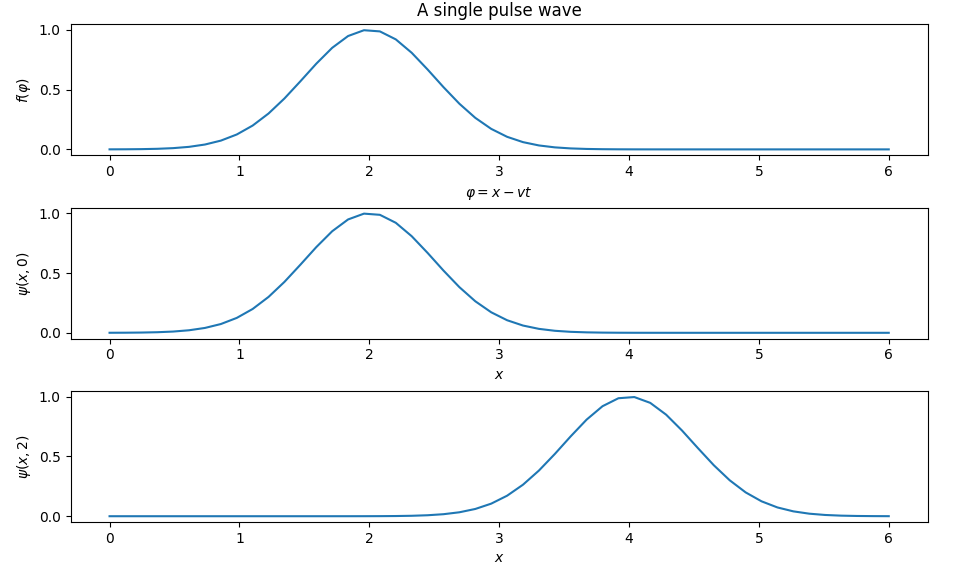
\includegraphics[scale=0.5]{pulse_wave.png}
        \caption{A function \(f\), the wave \(\psi(x, t) = f(x - vt)\) at times \(t = 0, 2\) for \(v = 1\).}
        \label{fig:pulse wave}
    \end{figure}
    The peak of \(f\) in this figure occurs at \(\varphi = x - vt = 2\).
    At \(t = 0\) we have \(\psi(x, 0) = f(x - 0)\) which has a peak at \(x = 2\).
    At \(t = 0\) we have \(\psi(x, 2) = f(x - 1\cdot 2)\) which still has a peak at \(\varphi = 2\) which means the peak is at \(x = 4\).
    We can also view this as a transformation of the original wave as \(x \to x - 2\) represents a translation \(+2\) units in the \(x\) direction.
    
    \subsubsection{Harmonic Wave}
    Often we think of waves as being periodic and repeating regularly.
    Of all the waves of this type the most important are the harmonic waves which are described mathematically by sines and cosines.
    We will see later that through Fourier series we can actually use a superposition of harmonic waves to describe any wave.
    
    The most simple harmonic wave is
    \[\psi(x, t) = A\sin(k(x - vt) - \Phi)\]
    where \(A\) is the amplitude, \(v\) is the velocity, and \(\Phi\) is some constant phase shift.
    The phase of this wave is \(\varphi = k(x - vt) - \Phi\).
    If we consider \(\psi\) at some fixed point as time varies we see it is periodic in time with period \(\tau\).
    We know that \(\sin\) is periodic with period \(2\pi\) so we must have that at \(x = x_0\)
    \[k(x_0 - vt_0) - \Phi - k(x_0 - v(t_0 + \tau)) + \Phi = 2\pi \implies kv = \frac{2\pi}{\tau} = \omega.\]
    \(\omega\) is the temporal angular frequency, or frequency for short.
    Similarly if we consider the wave at \(t = 0\) then we see that it is periodic in space with period \(\lambda\), known as the wavelength.
    Again \(\sin\) is periodic with period \(2\pi\) so
    \[k\lambda = 2\pi \implies k = \frac{2\pi}{\lambda}.\]
    \(k\) is the spatial angular frequency, or wave number for short.
    
    It is common to write waves in a way which explicitly gives \(k\) and \(\omega\), such as
    \[\psi(x, t) = A\sin(kx - kvt - \Phi) = A\sin(kx - \omega t - \Phi).\]
    This is beneficial as it puts space and time on an equal footing.
    We can easily recover \(v = \omega / k\).
    The relationship between spatial and temporal parts is called a \define{dispersion relation}.
    
    Another notational convenience is to use complex exponentials, such as
    \[\psi(x, t) = Ae^{i(kx - \omega t - \Phi)} = A\cos(kx - \omega t - \Phi) + i\sin(kx - \omega t - \Phi).\]
    The complex numbers simplify a lot of calculations but it is the real part of \(\psi\) that corresponds to the physical disturbance.
    
    \subsubsection{Phase Velocity}
    Strictly speaking the velocity of the wave that we have spoken of so far is the \define{phase velocity}.
    It is the velocity of a peak of the wave.
    For example the peak of our sinusoidal wave occurs at phase \(\varphi = \pi / 2\).
    If there is a crest at \((x_1, t_1)\) then we must have
    \[kx_1 - \omega t_1 - \Phi = \frac{\pi}{2}.\]
    At time \(t_1 + \delta t\) the crest must then be at \(x_1 + \delta x\) which satisfies
    \[k(x_1 + \delta x) - \omega(t_1 + \delta t) - \Phi = \frac{\pi}{2}.\]
    Subtracting the first of these from the second we get
    \[k\delta x - \omega\delta t = 0 \implies \frac{\delta x}{\delta t} = \frac{\omega}{k}.\]
    It is this velocity that we refer to when we say the phase velocity.
    Note that we don't have to use a crest here, we could just as well have used a trough or a point of zero displacement or any other condition of constant phase.
    
    \subsection{Waves in Three Dimensions}
    The wave equation generalises to three dimensions as
    \[\laplacian\psi = \frac{1}{v^2}\pdv[2]{\psi}{t},\]
    and the condition \(\psi(x, t) = f(kx - \omega t)\) becomes \[\psi(\vv{r}, t) = f(\vv{k}\cdot\vv{r} - \omega t),\]
    where \(\vv{k}\) is the \define{wave vector}.
    
    \subsubsection{Plane Waves}
    The quantity \(\vv{k}\cdot\vv{r}\) is the displacement in the direction \(\vv{k}\).
    There is a whole plane of points, \(\vv{r}\), which give the same value for \(\vv{k}\cdot\vv{r}\).
    These planes which satisfy \(\vv{k}\cdot\vv{r} = \text{const}\) are called wavefronts.
    These planes have the same phase everywhere on the plane at any given time.
    As well as the shape of the wavefronts we also have to consider the shape of the wave.
    one of the most common plane waves is
    \[\psi(\vv{r}, t) = Ae^{i(\vv{k}\cdot\vv{r} - \omega t - \Phi)}.\]
    
    Three-dimensional waves are hard to draw as we really need four dimensions to draw them, one for each spatial direction and one for the amplitude, even if we fix \(t\) as some constant value.
    Instead we will often consider a two-dimensional wave and use the third dimension for plotting the amplitude.
    For example see figure~\ref{fig:2d wave}.
    \begin{figure}[ht]
        \centering
        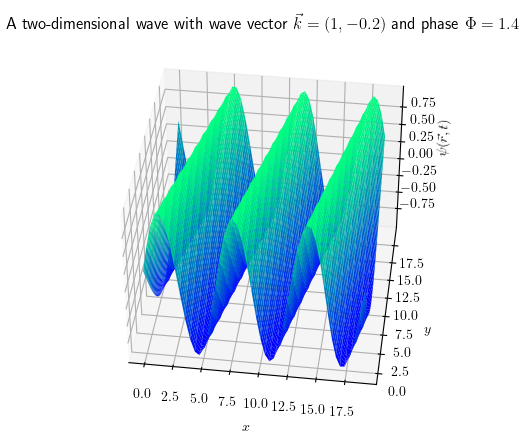
\includegraphics[scale=0.6]{2d_wave.png}
        \caption{A plane wave in two dimensions with \(\vv{k} = (1, -0.2)\) and \(\Phi = 1.4\). The wave is \(\psi(\vv{r}, t) = \exp(i[x - 0.2 y - 1.4])\).}
        \label{fig:2d wave}
    \end{figure}
    
    \subsubsection{Spherical Waves}
    Another common case of three-dimensional waves is something radiating from a point.
    In this case the wavefronts are spherical and we are best to work with spherical coordinates.
    The Laplacian of a central function in spherical coordinates is
    \[\laplacian\psi(r) = \frac{1}{r}\pdv{r}\left(r^2\pdv{\psi}{r}\right) = \pdv[2]{\psi}{r} + \frac{2}{r}\pdv{\psi}{r} = \frac{1}{r}\pdv[2]{r}(r\psi).\]
    Using the last version we find that \(r\psi\) satisfies the one-dimensional wave equation and therefore
    \[\psi(r, t) = \frac{1}{r}f(r - vt).\]
    For example a harmonic spherical wave might be given by
    \begin{equation}\label{eqn:harmonic spherical wave}
        \psi(r, t) = \frac{A}{r}\sin(k(r - vt)).
    \end{equation}
    The factor of \(1/r\) is important.
    It ensures that the intensity of the wave decreases as the wave spreads out.
    Far from the origin a spherical wave will approximate a plane wave.
    This can be seen in figure~\ref{fig:spherical wave approx plane wave}
    \begin{figure}[ht]
        \centering
        \tikzsetnextfilename{spherical-wave-approximates-plane-wave}
        \begin{tikzpicture}
            \begin{scope}[scale=0.8]
                \clip (-3, 0) rectangle (16, 4);
                \foreach \r in {0, ..., 16} {
                    \draw (1, 2) circle[radius=\r];
                }
                \draw[gray, dashed] (15.874, 4) -- (15.874, 0);
            \end{scope}
        \end{tikzpicture}
        \caption{A spherical wave at large distances approximates a plane wave. Notice how at the far right the wavefront is almost parallel to the straight dashed line.}
        \label{fig:spherical wave approx plane wave}
    \end{figure}

    \section{Electromagnetic Waves}
    \subsection{Energy Density and Optical Intensity}
    Recall that the Poynting vector is defined as
    \[\vv{S} = \frac{1}{\mu_0}\vv{E}\times\vv{B},\]
    and that the energy density of an electromagnetic wave in a vacuum is
    \[u = \frac{1}{2}\varepsilon_0E^2 + \frac{1}{2\mu_0}B^2 \varepsilon_0E^2.\]
    For a harmonic wave polarised in the \(x\) direction (that is \(\vv{E}\propto\ve{x}\) so \(\vv{B}\propto\ve{y}\) and \(\vv{k}\propto\ve{z}\)) the energy density is
    \[u = \varepsilon_0E^2 = \varepsilon_0 E_0^2\cos^2(kz - \omega t - \Phi)\]
    and the Poynting vector is
    \[\vv{S} = c\varepsilon_0E_0^2\cos^2(kz - \omega 6 - \Phi)\ve{z} = cu\ve{z}.\]
    For an optical wave \(\omega \approx \SI{e15}{\second^{-1}}\).
    It is therefore not possible to measure an instantaneous value of \(\vv{E}\), \(\vv{B}\), \(\vv{S}\), or \(u\).
    Instead we can measure the rate of energy transferred over a long period.
    This corresponds to averaging over many periods.
    We define the \define{intensity} as
    \[I = \expected{S} = c\varepsilon_0\expected{E}\]
    where \(\expected{f}\) denotes an average of \(f\) over many periods which can be computed as
    \[\expected{f} = \frac{1}{t_{\max}} \int_0^{t_{\max}}f(t)\dd{t}\]
    where \(t_{\max}\gg T\) where \(T = 2\pi/\omega\) is the period of \(f\).
    
    \subsection{Violation of Newton's Third Law?}
    Consider the two charges shown in figure~\ref{fig:violation of N3 setup}.
    \begin{figure}[ht]
        \centering
        \tikzsetnextfilename{moving-charges-violate-N2}
        \begin{tikzpicture}
            \tikzstyle{charge} = [fill=blue, color=blue]
            \tikzstyle{vector} = [very thick, ->]
            \draw[charge] (0, 0) circle[radius=0.2cm];
            \draw[charge] (4, 0) circle[radius=0.2cm];
            \node[above] at (0, 0.2) {\(q\)};
            \node[above] at (4, 0.2) {\(q\)};
            \draw[vector] (0, 0) -- (2, 0);
            \draw[vector] (4, 0) -- (4, -2);
            \node[right] at (2, 0) {\(\vv{v_1}\)};
            \node[below] at (4, -2) {\(\vv{v_2}\)};
            \draw[vector] (5, 0) -- (5, 1);
            \draw[vector] (5, 0) -- (6, 0);
            \node[above] at (5, 1) {\(z\)};
            \node[right] at (6, 0) {\(x\)};
            \draw[|-|] (0, 1) -- (4, 1);
            \node[above] at (2, 1) {\(d\)};
        \end{tikzpicture}
        \caption{Two moving charges.}
        \label{fig:violation of N3 setup}
    \end{figure}
    It shows two charges of charge \(q\).
    One is moving horizontally along the \(x\)-axis with velocity \(\vv{v_1}\) and the other is moving in the \(-z\) direction with velocity \(\vv{v_2}\).
    Suppose that \(v_1 = v_2 = v\).
    The force due to the electric field from charge 1 on charge 2 is
    \[\vv{F_{E2}} = \frac{q^2}{4\pi\varepsilon_0d^2}\ve{x}.\]
    Similarly the force due to the electric field from charge 2 on charge 1 is
    \[\vv{F_{E1}} = -\frac{q^2}{4\pi\varepsilon_0d^2}\ve{x}.\]
    These forces are equal and opposite as Newton's third law would predict.
    
    The force due to the magnetic field from charge 1 on charge 2 is
    \[\vv{F_{B2}} = q\vv{v_2}\times\vv{B_1} = q\vv{v_2}\times\left[\frac{q}{4\pi\varepsilon_0c^2}\frac{\vv{v_1}\times\vv{r_2}}{r_2^3}\right] = \vv{0}.\]
    This is \(\vv{0}\) since \(\vv{r_2}\), the vector from charge 1 to charge 2, is parallel to \(\vv{v_1}\).
    The force due to the magnetic field form charge 2 on charge 1 is
    \[\vv{F_{B1}} = q\vv{v_1}\times\vv{B_2} = q\vv{v_1} \times \left[\frac{q}{4\pi\varepsilon_0c^2}\frac{\vv{v_2}\times\vv{r_1}}{r_1^3}\right]\ne \vv{0}.\]
    So the forces due to the magnetic fields are \emph{not} equal and opposite.
    This seems to violate Newton's third law.
    In the next system we will see why this is.
    
    \subsection{Radiation Pressure}
    Light incident on a positive charge, \(q\), at some moment when \(\vv{E}\) is in the positive \(x\) direction will initiate movement of the charge in the positive \(x\) direction doing work at a rate
    \[\dv{W}{t} = \vv{v}\cdot\vv{F_E} = v_xqE_x.\]
    At this point the charge is moving and therefore experiences a force due to the magnetic component of the light.
    At the same moment this component is in the positive \(y\) direction and the force is
    \[\vv{F_B} = q\vv{v}\times\vv{B} = qv_x\ve{x}\times B_y\ve{y} = qv_xB_y\ve{z}.\]
    At a later time when \(\vv{E}\) is in the negative \(x\) direction the rate of work that \(\vv{E}\) does will be
    \[\dv{W}{t} = \vv{v}\cdot\vv{F_E} = -v_xqE_x.\]
    At the same moment \(\vv{B}\) will be in the negative \(y\) direction and the charge will be moving now in the negative \(x\) direction so the force due to the magnetic field is
    \[\vv{F_B} = q\vv{v}\times\vv{B} = q(-v_x\ve{x})\times(-B_y\ve{y}) = qv_xB_y\ve{z}.\]
    Notice that one period the average force due to \(\vv{E}\) is 
    \[\expected{\vv{F_E}} = q\expected{\vv{E}} = \vv{0}.\]
    However the average net force is
    \[\expected{\vv{F}} = \expected{\vv{F_E} + \vv{F_B}} = \expected{\vv{F_B}} = q\expected{v_xB_y}\ve{z} = \frac{q}{c}\expected{v_xE_x}\ve{z},\]
    using the fact that for an electromagnetic wave \(B_y = E_x/c\).
    From this we see that there is a net force which does work at a rate
    \[\expectedResize{\dv{W}{t}} = \expected{\vv{v}\cdot\vv{F}} = \expected{\vv{v}\cdot(\vv{F_E}\cdot\vv{F_B}} = \expected{\vv{v}\cdot\vv{F_E}} = q\expected{v_xE_x},\]
    where we have used the fact that \(\vv{v}\cdot\vv{F_B} = \vv{v}\cdot(\vv{v}\times\vv{B}) = 0\).
    We see that there is a net gain in energy while the light is incident on the charge.
    Notice that
    \[\expectedResize{\dv{W}{t}}\ve{z} = c\expected{\vv{F}} = \expectedResize{\dv{\vv{p}}{t}}.\]
    So there is a net gain in momentum.
    This gain of momentum is inversely proportional to \(c\) so is often too small to notice.
    The pressure due to this force is called \define{radiation pressure}.
    For example on Earth the energy density from solar radiation is approximately \(\SI{1}{\kilo\watt.\meter^-2}\).
    This is an appreciable amount of energy, the sun feels warm.
    However the radiation pressure is then on the order of \(\SI{e-6}{\pascal}\) which is 11 orders of magnitude smaller than atmospheric pressure.
    
    While this effect is small it is still important.
    For example there have been a few space probes that use the radiation pressure of the sun to accelerate.
    To do this they use large sails to maximise the are over which sunlight is incident.
    Even traditionally driven probes have to account for the radiation pressure changing their course slightly.
    
    This effect also explains the seeming violation of Newton's third law earlier.
    If we properly account for the radiation pressure then we will find that Newton's third law is not violated.
    
    We saw with radiation pressure that the momentum is equal to the energy divided by \(c\).
    If we consider for a moment quantum mechanics then we have
    \[p = \frac{h}{\lambda}\qquad \text{and} E = hf = \frac{hc}{\lambda} = pc \implies p = \frac{E}{c}.\]
    If instead we consider special relativity then we have
    \[E^2 = m^2c^4 + p^2c^2\]
    if \(m = 0\) then we have
    \[E = pc \implies p = \frac{E}{c}.\]
    So we have agreement between electromagnetism, quantum mechanics, and special relativity as to \(p = E/c\).
    
    One experimental verification of radiation pressure comes from Compton scattering.
    This is a process by which an incoming photon of wavelength \(\lambda_i\) hits an electron which deflects away at angle \(\varphi\) and the photon deflects at angle \(\vartheta\).
    The wavelength of the scattered photon is \(\lambda_f\).
    It can be shown that
    \[\lambda_f - \lambda_i = \Delta \lambda = \frac{h}{m_ec}(1 - \cos\vartheta).\]
    Since some momentum must be transferred to the electron the momentum of the photon must decrease and therefore the wavelength changes.
    
    \section{Dipole Radiation}
    \subsection{Light From Maxwell's Equations}
    Recall that we can combine Maxwell's equations to get the wave equations
    \[\laplacian\vv{E} = \mu_0\varepsilon_0 \partial_t^2\vv{E}, \qquad\text{and}\qquad \laplacian\vv{B} = \mu_0\varepsilon_0\partial_t\vv{B}.\]
    We see that each component of the electric and magnetic fields must satisfy the three-dimensional wave equation for a wave travelling at speed \((\mu_0\varepsilon_0)^{-1/2}\), which is the speed of light.
    This was one of the facts that originally convinced Maxwell that light could be explained as an electromagnetic phenomenon.
    
    Suppose we have an electromagnetic wave which propagates such that
    \[E_i(\vv{r}, t) = f(\vv{k}\cdot\vv{r} - \omega t).\]
    These are plane waves propagating along \(\vv{k}\).
    Now we choose \(\ve{z}\) to be the same direction as \(\vv{k}\) so that \(E_i(\vv{r}, t) = f(kz - \omega t)\).
    We see that
    \[\div\vv{E} = \partial_z E_z\]
    if we further assume that the wave is propagating in free space then we have \(\div\vv{E} = 0 = \partial_z E_z\).
    This means that \(\vv{E}\) doesn't oscillate in the direction of propagation meaning that it is a transverse wave.
    Suppose at some point \(\vv{E}\) is aligned with \(\ve{x}\).
    Then We must have \(\vv{B}\) parallel to \(\ve{y}\) as we know that it is perpendicular to \(\vv{E}\).
    
    Suppose
    \[\vv{E} = E_x(\vv{r}, t)\ve{x} = E_{x0}\cos(kz - \omega t - \Phi)\ve{x}.\]
    That is \(\vv{E}\) is a harmonic wave polarised in the \(x\) direction.
    We then find from Faraday's law that
    \[-\partial_t B_y = \partial_z E_x = -E_{x0}k\sin(kz - \omega t - \Phi).\]
    From this we have
    \[B_y = E_{x0}k \int \sin(kz - \omega t - \Phi) \dd{t} = E_{x0}\frac{k}{\omega}\cos(kz - \omega t - \Phi) = \frac{1}{c}E_{x0}\cos(kz - \omega t - \Phi) = \frac{E_x}{c}.\]
    So the \(\vv{B}\) oscillates perpendicular to \(\vv{E}\) and has a magnitude \(B = E/c\).
    
    \subsection{Dipole Radiation}
    Suppose we have an atom at rest.
    If we displace the electron cloud slightly we will have an effective dipole.
    This dipole turns out to be critical to how light interacts with matter.
    Suppose that we distort an atom to create a dipole moment \(\vv{p_0}\).
    Approximating this as an ideal dipole the field we expect is
    \[E_r = \frac{2p_0\cos\vartheta}{4\pi\varepsilon_0r^3}, \qquad\text{and}\qquad E_\vartheta = \frac{p_0\sin\vartheta}{4\pi\varepsilon_0r^3}.\]
    Due to rotational symmetry about \(\vv{p_0}\) we expect that there will be no \(\varphi\) dependence of the field.
    
    If we slightly distort the dipole and then allow it to change freely then to second order we expect harmonic oscillation so we expect the dipole to vary as
    \[\vv{p}(t) = \vv{p_0}\cos(\omega t).\]
    However we cannot use this new dipole in the equations for a dipole field.
    The problem is that these equations assume the dipole is static, which is no longer the case.
    The reason this assumption is necessary is the finite speed of light.
    While the dipole oscillates it takes time for the change in the field to propagate and by the time it has the dipole is different again.
    There is a time lag in the response to the oscillation and the lag increases with distance.
    
    \subsubsection{Retarded Time}
    The solution to the dipole field of an oscillating dipole uses a concept called \define{retarded time}.
    The retarded time at a distance \(x\) from an accelerating charge is \(t' = t - x/c\) where \(t\) is the actual time.
    We use square brackets, \([\cdot]\), to denote a quantity that is to be calculated at the retarded time.
    For example if \(a = a(t)\)  is the acceleration of a charge then \([a] = a(t')\) is the acceleration of the charge at the retarded time.
    If we have a single charge accelerating along the \(z\)-axis then it can be shown that the electric field at some distance, \(x\), along the \(x\)-axis at time \(t\) is
    \[\vv{E}(x, y=0, z=0, t) = \ve{x}\frac{q}{4\pi\varepsilon_0 x^2} - \ve{z}\frac{q[a]}{4\pi\varepsilon_0 xc^2}.\]
    The first term is the normal Coulomb term due to the presence of the charge.
    The second term, called the retarded term, is due to the accelerating charge causing a changing magnetic field which in turn causes an electric field.
    We see that in the limit \(c\to\infty\) the retarded term disappears which makes sense since the retarded term only appears due to the fact that \(c\) is \emph{not} infinite.
    In the limit \(x\to\infty\) the retarded term dominates.
    
    \subsubsection{Full Dipole Radiation Equations}
    It can be shown that the electric and magnetic fields for a time dependent dipole, with magnitude \(p(t)\) oriented along the \(z\)-axis, are given by
    \begin{align*}
        E_r &= \frac{2}{4\pi\varepsilon_0} \left(\frac{[p]}{r^3} + \frac{[\inlinedv{p}{t}]}{cr^2}\right),\\
        E_\vartheta &= \frac{1}{4\pi\varepsilon_0} \left(\frac{[p]}{r^3} + \frac{[\inlinedv{p}{t}]}{cr^2} + \frac{[\inlinedv[2]{p}{t}]}{c^2r} \right) \sin\vartheta,\\
        B_\varphi &= \frac{1}{4\pi\varepsilon_0} \left(\frac{[\inlinedv{p}{t}]}{c^2r^2} + \frac{[\inlinedv[2]{p}{t}]}{c^3r}\right) \sin\vartheta
    \end{align*}
    and
    \[E_\varphi = B_r = B_\vartheta = 0.\]
    The terms including a factor of \([p]\) are the fields due to the static field.
    Again if we take the limit \(c\to\infty\) then this reduces to the equations for a static dipole as propagation time becomes zero.
    Far from the dipole the \(1/r^3\) terms dominate and we have
    \[E_r\approx 0, \qquad E_{\vartheta} \approx \frac{1}{4\pi\varepsilon_0} \frac{[\inlinedv[2]{p}{t}]}{c^2r}\sin\vartheta, \qquad\text{and}\qquad B_\varphi \approx \frac{1}{4\pi\varepsilon_0} \frac{[\inlinedv[2]{p}{t}]}{c^3r}\sin\vartheta.\]
    These equations are much simpler and we will work with them.
    We see that \(B = E/c\) as we would expect and also that \(\vv{E}\) and \(\vv{B}\) are perpendicular to each other and to \(\ve{r}\) which is the propagation direction.
    The two fields are in phase and the \(\sin\vartheta\) term means that the fields are strongest around the `equator' of the dipole and are zero along the \(z\) axis.
    The \(\vv{B}\) field is azimuthal (in the \(\ve{\varphi}\) direction) which is also the case with a current carrying wire along the \(z\)-axis.
    Far from the origin \(\vv{E}\) and \(\vv{B}\) have a form similar to  equation~\ref{eqn:harmonic spherical wave} which means that they look like harmonic spherical waves with an extra \(\sin\vartheta\) term which decreases the magnitude towards the poles.
    As one last observation note that the magnitude of the pointing vector is \(S = \abs{\mu_0^{-1}\vv{E}\times\vv{B}} \propto 1/r^2\), so intensity decays as \(I = \expected{S} \propto 1/r^2\) as we would expect for light which famously follows an inverse square law for intensity.
    
    All of these points hold for the approximate version of the equations `far' from the dipole.
    So when is this a good approximation?
    What counts as far?
    The answer turns out to be that far is not very far at all.
    In fact the \(1/r\) terms dominate enough that the approximation is valid for \(r\) being only a few wavelengths which is very small.
    Since the approximation is valid so close and we aren't doing quantum mechanics we really needn't consider anything other than the far field approximation here.
    
    \section{Electromagnetic Waves in Dielectrics}
    An electromagnetic field in a dielectric with permittivity \(\varepsilon = \varepsilon_0\varepsilon_r\) and permeability \(\mu = \mu_0\mu_r\) can be shown to lead to the wave equations
    \[\laplacian\vv{E} = \varepsilon\mu\partial_t^2\vv{E}, \qquad\text{and}\qquad \laplacian\vv{B} = \varepsilon\mu \partial_t^2\vv{B}.\]
    We assume that the dielectric is linear, isotropic and homogenous.
    That is the polarisation is linearly proportional to the applied electric field and the material properties are the same in all directions and everywhere in space.
    
    These corresponds to waves with phase velocity
    \[v_p = \frac{\omega}{k} = \frac{1}{\sqrt{\mu\varepsilon}} = \frac{c}{\sqrt{\mu_r\varepsilon_r}}.\]
    We see that the speed of light in the medium is attenuated by a factor of \(1/\sqrt{\mu_r\varepsilon_r}\).
    We call this factor, \(n = \sqrt{\mu_r\varepsilon_r}\), the \define{refractive index}.
    For a material that is not a ferromagnet we find that \(\mu_r \approx 1\) and so \(n = \sqrt{\varepsilon_r}\) is usually a good approximation for our purposes and
    \[v_p = \frac{c}{\sqrt{\mu_r\varepsilon_r}} = \frac{c}{n} \approx \frac{c}{\sqrt{\varepsilon_r}}.\]
    
    Recall that an electric field causes a polarisation \(\vv{P} = \chi_E\varepsilon_0\vv{E}\) where \(n^2 \approx \varepsilon_r = 1 + \chi_E\).
    Therefore if we can calculate the polarisation, \(\vv{P}\), we can find \(\varepsilon_r\) and from this we can find the refractive index, \(n\).
    We can calculate \(\vv{P}\) from the polarisation of a single molecule, \(\vv{p}\), and then \(\vv{P} = N\vv{p}\) where \(N\) is the number density of molecules.
    
    \subsection{Snell's Law Derivation From Fermat's Principle}\label{sec:snell's law fermat's principle}
    Fermat's principle of stationary time states that a light ray travelling between two points takes a path such that the time taken is stationary with respect to variations in the path.
    Roughly speaking this means that a slight variation in the path to a nearby path will cause, at most, second order changes in the traversal time.
    While the principle simply states `stationary' it is often assumed that the time taken is in fact minimal.
    After all there is an infinite number of paths that take arbitrarily long to reach the point.
    
    Fermat's principle makes no assumptions about light as an electromagnetic wave but we will see that it leads to many correct predictions.
    For example, we will use it here to derive Snell's law.
    This principle is the basis of geometric optics, which is the field of optics where light is treated as a ray and its path through space calculated based on various rules for how this ray interacts with the mediums it travels through.
    
    \begin{figure}[ht]
        \centering
        \tikzsetnextfilename{refraction-again}
        \begin{tikzpicture}
            \tikzstyle{glass} = [fill=blue!50, opacity=0.3, color=blue!50]
            \tikzstyle{ray} = [very thick, red, decoration={markings, mark=at position 0.5 with {\arrow{>}}}, postaction={decorate}]
            \draw[glass] (-2, -2) rectangle (3, 0);
            \draw[dashed, thick] (1, -2) -- (1, 2);
            \draw[thick, ->] (-1, -2) -- (-1, 2) node[above] {\(y\)};
            \draw[thick, ->] (-2, 0) -- (3, 0) node[right] {\(x\)};
            \node at (-1.8, 0.3) {\(n_1\)};
            \node at (-1.8, -0.3) {\(n_2\)};
            \draw[ray] (-1, 1.5) -- (1, 0);
            \draw[ray] (1, 0) -- (2, -2);
            \draw[fill=black] (1.75, -1.5) circle[radius=0.05cm] node[right] {\(B = (a, -b)\)};
            \draw[fill=black] (-1, 1.5) circle[radius=0.05cm] node[left] {\(A = (0, b)\)};
            \begin{scope}
                \clip (1, 0) -- (1, 2) -- (-1, 1.5) -- (1, 0);
                \draw (1, 0) circle[radius=0.5cm];
            \end{scope}
            \node at (0.75, 0.65) {\(\vartheta_i\)};
            \begin{scope}
                \clip (1, 0) -- (2, -2) -- (1, -2) -- (1, 0);
                \draw (1, 0) circle[radius=0.5cm];
            \end{scope}
            \node at (1.2, -0.7) {\(\vartheta_r\)};
        \end{tikzpicture}
        \caption{Light being refracted at the boundary between two media.}
        \label{fig:snell's law by fermat's principle}
    \end{figure}
    Consider light travelling from point \(A\) to \(B\) and along the way it changes from one medium with refractive index \(n_1\) to another with refractive index \(n_2\).
    Within a medium the only stationary path is a straight line, which is what we expect.
    What we don't know is what angles the light will meet the medium at.
    It is traditional to consider the angle to the normal with the incoming angle being called the angle of incidence, \(\vartheta_i\), and the outgoing angle being called the angle of refraction, \(\vartheta_r\)
    Set up coordinates as in figure~\ref{fig:snell's law by fermat's principle}.
    Notice that the diagram shows \(\vartheta_r < \vartheta_i\) but this is not necessarily the case.
    We can fix both angles by choosing the point \(C = (x, 0)\), along the \(x\)-axis at which the light passes from one medium to the other.
    
    The total time taken for the light to travel from \(A\) to \(B\) is \(T = T_1 + T_2\) where \(T_1\) is the time to travel the path in medium 1 and \(T_2\) is the time to travel the path in medium 2.
    Using the fact that the speed of light in a given medium is \(c/n_i\) and the fact that time is distance over speed we have
    \begin{align*}
        T &= T_1 + T_2\\
        &= \frac{\abs{\overrightarrow{AC}}}{c/n_1} + \frac{\abs{\overrightarrow{CB}}}{c/n_2}\\
        &= \frac{\sqrt{b^2 + x^2}}{c/n_1} + \frac{\sqrt{b^2 + (a - x)^2}}{c/n_2}.
    \end{align*}
    For the time to be stationary we require
    \[\dv{T}{x} = 0.\]
    Calculating the derivative we have
    \[\dv{T}{x} = \frac{n_1}{c} \frac{x}{\sqrt{b^2 + x^2}} - \frac{n_2}{c} \frac{a - x}{\sqrt{b^2 + (a - x)^2}} = 0.\]
    Hence
    \[\frac{n_1x}{\sqrt{b^2 + x^2}} = \frac{n_2(a - x)}{\sqrt{b^2 + (a - x)^2}}.\]
    Now simply applying the definition of \(\sin\vartheta\) as opposite over hypotenuse we have
    \[n_1\sin\vartheta_i = n_2\sin\vartheta_r.\]
    This is \define{Snell's law} of refraction.
    This derivation was based on geometric optics and Fermat's principle of stationary time.
    In later sections we will derive this same result with Huygen's principle and full electromagnetic theory.
    
    \subsection{Polarisation and Refractive Index}
    We can use Snell's law to measure the refractive index of a material.
    If we do this we find that \(n\) decreases as frequency decreases.
    If we ask why this is the first thing we may think of is since \(n^2 = \varepsilon_r\) is related to polarisation the polarisation must also be frequency dependent.
    To find out why we may ask what it is that causes polarisation.
    There are three components that we might consider:
    \begin{itemize}
        \item The orientation of polar molecules leads to polarisation when the molecules align their dipoles with the electromagnetic field.
        This requires the entire molecule to rotate so happens on the time scales of rotational frequencies.
        For example in water it takes approximately \SI{10}{\pico\second}.
        \item The polarisation of ions leads to polarisation when the molecules distort to align the resulting dipole with the electromagnetic field.
        This requires only part of the molecule to move and so happens on the time scale of vibrational frequencies.
        For example in water it takes approximately \SI{1}{\pico\second}.
        \item The polarisation of non-polar molecules leads to polarisation when the electron cloud is distorted to create a dipole aligned with the electromagnetic field.
        This requires only electrons to move and so happens on very short time scales of about \SI{1}{\femto\second}.
    \end{itemize}
    From all of these mechanisms the key point is that polarisation is not instantaneous.
    If the field is oscillating back and forth we expect the polarisation to lag behind.
    How much it lags behind will depend on how fast the field oscillates.
    There si just one problem.
    This explanation would lead to us expecting that refractive index decreases as frequency increases.
    This is the exact opposite of what we see experimentally.
    To find out why this isn't what happens we will need a more careful treatment of the oscillation of the dipoles with changes in the field.
    This is what we will do in the next section.
    
    \section{Oscillator Model}
    For simplicity we assume that interactions between electrons are negligible and that we can model the electron cloud as simply being stuck in a potential well caused by the Coulomb interaction with the nucleus.
    If we expand this potential to second order then, by definition, we have a quadratic potential.
    We can therefore model the motion of the electron cloud as a harmonic oscillator obeying
    \[\massElectron \dv[2]{x}{t} = \chargeElectron E_x - \massElectron\omega_0^2x - \massElectron\gamma \dv{x}{t}.\]
    Here \(\massElectron\) and \(\chargeElectron\) are the mass and charge of the electron cloud, \(x\) is the displacement of the centre of mass of the electron cloud from the centre of mass of the atom and \(\gamma\) is a damping coefficient.
    We also assume that any radiation is \(x\) polarised for simplicity so
    \[E_x = E_0\cos(\omega t).\]
    If we include this we then have a damped harmonic oscillator with resonant frequency \(\omega\) being driven at frequency \(\omega\).
    
    In the undamped (\(\gamma = 0\)) case this has the solution
    \[x(t) = x_0\cos(\omega t) = \frac{\chargeElectron/\massElectron}{\omega_0^2 - \omega^2}E_i\cos(\omega t) = \frac{\chargeElectron/\massElectron}{\omega_0^2 - \omega^2}E(t).\]
    Notice that this motion of the electron cloud sets up a dipole with dipole moment \(p = \chargeElectron x\).
    Notice also that \(\chargeElectron < 0\) and the dipole vector, \(\vv{p}\), is conventionally defined to point from negative to positive, meaning that \(\vv{p}\) points in the opposite direction to \(\vv{x}\).
    From this we can draw conclusions based on two different cases for the values of \(\omega\) and \(\omega_0\):
    \begin{itemize}
        \item For the case of \(\omega < \omega_0\), i.e. below the natural frequency, the electron shell oscillates exactly \(\pi\) out of phase with the electric field, \(\vv{E}(t)\).
        That is \(\vv{x}\) points in the opposite direction to \(\vv{E}\) and so \(\vv{p}\) points in the same direction to \(\vv{E}\).
        
        \item For the case of \(\omega > \omega_0\), i.e. above the natural frequency, the electron cloud oscillates exactly in phase with the electric field, \(\vv{E}(t)\).
        That is \(\vv{x}\) points in the same direction as \(\vv{E}\) and so \(\vv{p}\) points in the opposite direction to \(\vv{E}\).
    \end{itemize}
    We can use the solution for \(x(t)\) to find the atomic dipole moment, \(\vv{p_{\mathrm{atom}}}\) and the polarisation of the atom, which is simply the dipole moment per unit volume.
    From this we can calculate the refractive index:
    \begin{align*}
        n^2 &= \varepsilon_r\\
        &= 1 + \frac{P}{\varepsilon_0E}\\
        &= 1 + \frac{Np_{\mathrm{atom}}}{\varepsilon_0E}\\
        &= 1 + \frac{N\chargeElectron x}{\varepsilon_0E}\\
        &= 1 + \frac{N\chargeElectron^2}{\varepsilon_0\massElectron (\omega_0^2 - \omega^2)}
    \end{align*}
    where \(N\) is the number density (i.e. the number of atoms per unit volume).
    
    This is a simple model so it won't give exactly the right solution.
    In particular it has the following shortcomings:
    \begin{itemize}
        \item In reality there won't be one single resonant frequencies but different components of motion will have different resonant frequencies, \(\omega_{0i}\), and we will have to sum over these.
        
        \item We ignore the interaction between atoms and in particular the effect that atomic dipole has on its neighbours.
        This can be accounted for with something called the Claussius--Mossotti correction but we won't take it into account.
        
        \item There is a singularity at \(\omega = \omega_0\).
    \end{itemize}
    
    In the case where we have non-zero damping the mathematics is harder but we can still find a solution.
    The correct damping regime to consider is light damping where \(0 < \gamma \ll 1/(2\omega_0)\).
    Recall that \(\gamma = 2\omega_0\) leads to critical damping.
    For non-zero damping the initial displacement at \(t = 0\) has explicit \(\omega\) dependence and a phase shift as well.
    The solution turns out o be of the form \(x = x_0\cos(\omega t + \Phi)\) leading to an atomic dipole of the form
    \[p_x = \chargeElectron x = p_0\cos(\omega t + \Phi)\]
    which can be shown to give solutions of the form
    \[p_0(\omega) = \chargeElectron x_0(\omega) = \frac{\chargeElectron^2 E_0/\massElectron}{\sqrt{(\omega_0^2 - \omega^2)^2 + \gamma^2\omega^2}}\]
    and
    \[\Phi = \arctan\left[ \frac{-\gamma\omega}{\omega_0^2 - \omega^2} \right].\] 
    We can solve this for \(x\) and it is easier to do this using complex exponentials for trig and we simply implicitly take the real part when necessary.
    Using \(x = x_0\exp[-i(\omega t + \Phi)]\) we find that
    \[x(\omega) = x_0e^{-i(\omega t + \Phi)} = x_0e^{-i\Phi}e^{-i\omega t} = \left[ \frac{\chargeElectron E_0/\massElectron}{\omega_0^2 - \omega^2 - i\gamma\omega} \right]e^{-i\omega t}\]
    and the dipole moment is then
    \[p_x(\omega) = \frac{\chargeElectron^2 E_x/\massElectron}{\omega_0^2 - \omega^2 - i\gamma \omega}.\]
    We then have
    \begin{equation}\label{eqn:epsilon r oscillator model}
        \varepsilon_r = \varepsilon_r' + i\varepsilon_r'' = 1 + \frac{N\chargeElectron^2}{\varepsilon_0\massElectron (\omega_0^2 - \omega^2 - i\gamma\omega)}
    \end{equation}
    where \(\varepsilon_r'\) and \(\varepsilon_r''\) are the real and imaginary components of \(\varepsilon_r\).
    Using a similar notation for the refractive index, \(n = n' + in''\) we have
    \[\varepsilon_r = n^2 \implies \varepsilon_r' = n'{^2} - n''{^2}, \qquad\text{and}\qquad \varepsilon_r'' = 2n'n''.\]
    Since \(\varepsilon_r\) depends on the frequency, \(\omega\), of the radiation we find that the refractive index also depends on the frequency of the radiation meaning that different colours of light are diffracted/refracted/slowed down by a different amount.
    We can also replace \(\omega_0^2\) with \(\omega_{01}^2 + \omega_{02}^2 + \dotsb\) where \(\omega_{0i}\) are the relevant natural frequencies of the oscillations.
    
    A few features of this new equation show us that it is a good model or raise some more questions:
    \begin{itemize}
        \item If \(\gamma \ne 0\) then we don't have any singularities, even at \(\omega = \omega_0\).
        
        \item The real part of the refractive index, \(n'\), increases with the frequency as \(\omega\) becomes closer to \(\omega_{0i}\) which is what we observe experimentally.
        
        \item Ignoring increases for \(\omega \approx \omega_{0i}\) we have a general decreasing trend in \(n'\) with \(\omega\).
        
        \item For \(\omega > \max\{\omega_i\}\) we have \(n' < 1\) which means that light at these frequencies travels faster than \(\SI{3e8}{\metre.\second^{-1}}\).
        This seems initially like it breaks the rules of special relativity until you recall that the speed of light applies only in a vacuum.
        
        \item Using this model we can measure refractive index dependent things at some frequencies and extrapolate to other frequencies.
    \end{itemize}

    \subsection{Interpreting the Oscillator Model}
    Consider the case of a free electron.
    This corresponds to setting \(\omega_0 = 0\) and so \(\omega_0 < \omega\) which we saw in the previous section meant that the electron oscillates in phase with \(\vv{E}\).
    This initially seems incorrect as the electron has a negative charge and so should move in the \emph{opposite} direction to \(\vv{E}\).
    This would indeed be the case if \(\vv{E}\) was constant, but it isn't.
    The \emph{acceleration} of the electron is what must be in the opposite direction of \(\vv{E}\).
    The displacement is then given by integrating twice and integrating a sinusoid twice gives, up to a positive constant factor, the same sinusoid back but negative.
    So the acceleration is in the opposite direction to \(\vv{E}\) but the position is in the same direction as \(\vv{E}\).
    
    If instead \(\vv{E}\) is static, or equivalently \(\omega = 0\), then the electron is displaced in the opposite direction to \(\vv{E}\) which agrees with the case of \(\omega < \omega_0\) (even though \(\omega = \omega_0 = 0\)).
    
    For the case of \(\omega \approx \omega_0\) we have a large spike in amplitude.
    In the case of the undamped oscillator this is a singularity and the amplitude becomes infinite.
    In the lightly damped case the amplitude is finite but still much larger than in other regions.
    This is due to resonance, recall that a harmonic oscillator has its maximum amplitude at some resonant frequency, \(\omega_r\), which is just slightly lower than \(\omega_0\).
    
    Consider the case of very light damping such that \(\gamma\) becomes infinitesimal.
    In this case the imaginary part of \(x\) or \(\varepsilon_r\) becomes a delta distribution at \(\omega_0\) and the real part becomes discontinuous.
    This is because there is no limit on vibration amplitude in this mathematical model.
    In a real material there is damping as oscillating dipoles will lose energy due to random thermal collisions.
    The dipoles will also re-radiate energy.
    This gives a physical significance the the complex parts of \(\varepsilon_r\) and \(n\) which up until now we have treated purely as a mathematical convenience.
    These terms correspond to how much a given frequency is absorbed by the medium.
    For example glass has \(\omega_0 \approx \SI{e6}{\radian.\second^{-1}}\), which corresponds to light in the UV region of the spectrum.
    Glass also strongly absorbs UV radiation at this frequency which corresponds to the high peak at this point in \(\varepsilon_r''\) and \(n''\).
    
    For low frequencies, \(\omega \ll \omega_0\), \(\tan\Phi\) is small and negative, which means that \(\Phi\) is small and negative.
    This means that the oscillations have a negligible phase lag.
    For \(\omega = \omega_0\) we have \(\Phi = -\pi/2\) and for \(\omega \gg \omega_0\) we \(\Phi\) approaches \(-\pi\).
    So the phase lag increases as \(\omega\) increases.
    This corresponds to \(\varepsilon_r\) dropping from greater than 1 for \(\omega \ll \omega_0\) to being smaller than 1 for \(\omega \gg \omega_0\).
    At low frequencies the polarisation of matter opposes the changing electric field and at higher frequencies it reinforces the changing field.
    
    
    \section{Huygens' Principle and Colour}
    \subsection{Huygens' Principle}\label{sec:huygens principle}
    So far we have considered electromagnetic radiation at a point propagating outwards from a dipole.
    We haven't seen how the fields from many dipole oscillators can combine to form an electromagnetic wave that fills space.
    The simplest explanation is called \define{Huygens' principle}:
    \begin{displayquote}
        Every point on a primary wavefront serves as the source of spherical secondary wavelets which travel at the speed of light such that the primary wavefront at some time later is the envelope of these wavelets.
    \end{displayquote}
    What this means is that every point emits waves which combine to form a new wave front.
    \begin{figure}[ht]
        \centering
        \tikzsetnextfilename{huygens-principle}
        \begin{tikzpicture}
            \draw[semithick] (0, 0) .. controls (1, 2) and (-1, 4) .. (0, 6);
            \foreach \i in {0, 0.05, ..., 1.05} {
                \draw[draw=none] (0, 0) .. controls (1, 2) and (-1, 4) .. (0, 6) coordinate[pos=\i] (A) {};
                \draw[fill=black] (A) circle[radius=0.05cm];
                \draw[lightgray] (A) circle[radius=0.5cm];
            }
            \draw[red] (0.5, 0) .. controls (1.5, 2) and (-0.5, 4) .. (0.5, 6);
            
            \begin{scope}[xshift=3cm]
                \draw[semithick] (0, 0) .. controls (1, 2) and (-1, 4) .. (0, 6);
                \foreach \i in {0, 0.05, ..., 1.05} {
                    \draw[draw=none] (0, 0) .. controls (1, 2) and (-1, 4) .. (0, 6) coordinate[pos=\i] (A) {};
                    \draw[fill=black] (A) circle[radius=0.05cm];
                    \begin{scope}
                        \clip (0.25, -0.5) -- (0.25, 0) .. controls (1.25, 2) and (-0.75, 4) .. (0.25, 6) -- (0.25, 6.5) -- (1, 6.5) -- (1, -0.5) -- cycle;
                        \draw[lightgray] (A) circle[radius=0.5cm];
                    \end{scope}
                }
            \end{scope}
        \end{tikzpicture}
        \caption{Many points along a wavefront emit wavelets which form a new wavefront.}
        \label{fig:huygens principle}
    \end{figure}
    This can be seen in figure~\ref{fig:huygens principle}.
    What isn't clear is why we only consider wavelets propagating in the forward direction.
    The reason for this will be given later when we have discussed superposition and interference.
    
    \subsection{Colour}
    As human beings we give particular attention to the visible part of the spectrum because, well, we can see it.
    The physics isn't fundamentally different for the rest of the spectrum but it is worth spending some time considering the visible spectrum and how we see light.
    
    There are two types of colour.
    There are \define{pure}/\define{spectral}/\define{chromatic} colours such as red, blue, green, yellow, etc.\@ which are formed of a single wavelength and there are colours, such as purple or brown, which are a mixture of other colours.
    The pure colours are the ones we see when we pass light through a prism and split it up into a rainbow.
    
    \tikzexternaldisable
    \begin{table}[ht]
        \centering
        \definecolor{wavelengthViolet}{rgb}{0.356, 0, 0.75}
        \definecolor{wavelengthBlue}{rgb}{0.213, 0, 1}
        \definecolor{wavelengthGreenBlue}{rgb}{0, 0.622, 0.935}
        \definecolor{wavelengthBlueGreen}{rgb}{0, 0.898, 0.804}
        \definecolor{wavelengthGreen}{rgb}{0, 1, 0}
        \definecolor{wavelengthYellowGreen}{rgb}{0.93, 1, 0}
        \definecolor{wavelengthYellow}{rgb}{1, 0.725, 0}
        \definecolor{wavelengthOrange}{rgb}{1, 0.499, 0}
        \definecolor{wavelengthRed}{rgb}{0.818, 0, 0}
        \definecolor{wavelengthMagenta}{rgb}{1, 0, 1}
        \definecolor{wavelengthCyan}{rgb}{0, 1, 1}
        \begin{tabular}{cllll}\hline
            Wavelength (\si{\nano\metre}) & Colour & & & Complementary Colour\\\hline
            400--435 & Violet & \tikz{\fill[fill=wavelengthViolet] (0, 0) rectangle (0.25, 0.25);} & \tikz{\fill[fill=wavelengthYellowGreen] (0, 0) rectangle (0.25, 0.25);} & Yellow-Green\\
            435--480 & Blue & \tikz{\fill[fill=wavelengthBlue] (0, 0) rectangle (0.25, 0.25);} & \tikz{\fill[fill=wavelengthYellow] (0, 0) rectangle (0.25, 0.25);} & Yellow\\
            480--490 & Green-Blue & \tikz{\fill[fill=wavelengthGreenBlue] (0, 0) rectangle (0.25, 0.25);} & \tikz{\fill[fill=wavelengthOrange] (0, 0) rectangle (0.25, 0.25);} & Orange\\
            490--500 & Blue-Green & \tikz{\fill[fill=wavelengthBlueGreen] (0, 0) rectangle (0.25, 0.25);} & \tikz{\fill[fill=wavelengthRed] (0, 0) rectangle (0.25, 0.25);} & Red\\
            500--560 & Green & \tikz{\fill[fill=wavelengthGreen] (0, 0) rectangle (0.25, 0.25);} & \tikz{\fill[fill=wavelengthMagenta] (0, 0) rectangle (0.25, 0.25);} & Magenta\\
            560--580 & Yellow-Green & \tikz{\fill[fill=wavelengthYellowGreen] (0, 0) rectangle (0.25, 0.25);} & \tikz{\fill[fill=wavelengthViolet] (0, 0) rectangle (0.25, 0.25);} & Violet\\
            580--595 & Yellow & \tikz{\fill[fill=wavelengthYellow] (0, 0) rectangle (0.25, 0.25);} & \tikz{\fill[fill=wavelengthBlue] (0, 0) rectangle (0.25, 0.25);} & Blue\\
            595--605 & Orange & \tikz{\fill[fill=wavelengthOrange] (0, 0) rectangle (0.25, 0.25);} & \tikz{\fill[fill=wavelengthGreenBlue] (0, 0) rectangle (0.25, 0.25);} & Green-Blue\\
            605--700 & Red & \tikz{\fill[fill=wavelengthRed] (0, 0) rectangle (0.25, 0.25);} & \tikz{\fill[fill=wavelengthCyan] (0, 0) rectangle (0.25, 0.25);} & Cyan\\\hline
        \end{tabular}
    \end{table}
    \tikzexternalenable
    
    While many colours exist as a pure, single wavelength this is not how humans perceive colour.
    The human eye has three types of cones which are cells that can detect light.
    Each type preferentially detects light at one of three different wavelengths corresponding to red, green, and blue light.
    The brain then interprets both which cones are activated and also how much they are activated and combines this information to give us colour vision.
    For example if the red and green cones are activated a lot and the blue cones aren't activated at all then we see yellow:
    \tikzexternaldisable
    \definecolor{r}{rgb}{1,0,0}
    \definecolor{g}{rgb}{0,1,0}
    \definecolor{rg}{rgb}{1,1,0}
    \[\tikz{\fill[fill=r] (0, 0) rectangle (0.25, 0.25);} + \tikz{\fill[fill=g] (0, 0) rectangle (0.25, 0.25);} = \tikz{\fill[fill=rg] (0, 0) rectangle (0.25, 0.25);}.\]
    \tikzexternalenable
    If instead red is activated a lot and blue is activated about half as much then we see a sort of pink-purple colour:
    \tikzexternaldisable
    \definecolor{b}{rgb}{0,0,0.5}
    \definecolor{rb}{rgb}{1,0,0.5}
    \[\tikz{\fill[fill=r] (0, 0) rectangle (0.25, 0.25);} + \tikz{\fill[fill=b] (0, 0) rectangle (0.25, 0.25);} = \tikz{\fill[fill=rb] (0, 0) rectangle (0.25, 0.25);}.\]
    \tikzexternalenable
    We use this to produce colour in screens.
    Each pixel of a screen actually produces red, green, and blue, colour (RGB) in varying amounts which combine to give the colours we see.
    The standard way for this to happen is for the amount of each colour to be given by an 8 bit number which allows for values from 0 to 255.
    So for three different colours there are \(256^3 = 2^{8^3} = 2^{24} = 16777216\) different combinations that can be shown.
    This is just one of many ways of telling a computer what colour to show, an equivalent way uses hexadecimal instead and each colour is a six digit hexadecimal number ranging from \(\mathrm{\#000000} = 0\) for none of any colour (black) to \(\mathrm{\# FFFFFF} = 16777215\) for all of each colour (white).
    This isn't really that different as we can split the hexadecimal number into three two digit hexadecimal numbers each of which can be translated into binary to give the same three number RGB colour definition.
    
    Another aspect that needs to be considered is that the cones don't all only activate at a single wavelength but at a range of wavelengths and these ranges all overlap to some extent so light of a single wavelength can stimulate more than one type of cone at once which is how we see pure colours that aren't red, green, or blue.
    
    There are many mechanisms by which an object that doesn't produce its own light can become coloured in white light.
    We will discuss two right now.
    The simplest is colour by absorption.
    For example \ce{Cu^{2+}} absorbs most light except blue-green light and so when we see something with lots of \ce{Cu^{2+}} ions most of the light that bounces off of it is blue-green so this is the colour we see the object.
    The second mechanism is more complicated and involves scattering light at different wave lengths different amounts in such a way that most colours are scattered away before reaching us.
    This is the mechanism by which the sky appears blue.
    Scattering in the atmosphere scatters higher frequencies the most the light leaving the sun is pretty much white and so if you look directly at the sun\footnote{don't do this} you will see white light.
    Looking near the sun you see red/yellow light that has been scattered only a little bit.
    Looking far from the sun you see blue light which has been scattered far from the sun.
    The only reason that the sky isn't purple (as this light is the most scattered) is because the sun doesn't actually produce much purple light.
    
    \part[Light at Boundaries -- Reflection and Refraction]{Light at Boundaries\\{\LARGE Reflection and Refraction}}
    \section{Laws of Reflection and Refraction}
    We are mostly interested in this part in light incident on a sudden boundary between materials with different refractive indices.
    We will assume that the boundaries are smooth (on the scale of the wavelength).
    Recall that the angle of incidence is defined as the angle the incoming light makes to the surface normal pointing out of the surface.
    Similarly the angle of reflection is the angle that the reflected light makes to the same normal and the angle of transmission is the angle the transmitted light makes to the surface normal pointing into the surface.
    
    \subsection{Snell's Law}
    We have seen already in section~\ref{sec:snell's law fermat's principle} a derivation of Snell's law which depended on Fermat's principle---that light minimises the time taken to travel between points.
    We can also derive the same law with a full treatment of the equations for electromagnetic waves.
    
    Consider a boundary between two media with surface normal \(\vv{e}\).
    Incident on this surface is light with wave vector \(\vv{k_i}\).
    We would expect in general that there will be both reflection and transmission.
    The wave vector, \(\vv{k_i}\), and the surface normal, \(\vv{e}\), define a plane, called the plane of incidence.
    For a smooth surface all reflected and transmitted light will still be in this plane.
    The equation of the incoming light is
    \[\vv{E_i} = \vv{E_{0i}} \cos(\vv{k_i} \cdot \vv{r} - \omega t)\]
    where \(\vv{E_{0i}}\) is the amplitude and \(\omega\) is the frequency of the light.
    The energy of light is proportional to \(\omega\) and so to conserve energy the reflected and transmitted light must have the same frequency as the incident light.
    This means that we can express the electric field of the reflected light as
    \[\vv{E_r} = \vv{E_{0r}} \cos(\vv{k_r} \cdot \vv{r} 0 \omega t - \Phi_r)\]
    where \(\Phi_r\) is some phase difference to be calculated.
    Similarly the transmitted field is given by
    \[\vv{E_t} = \vv{E_{0t}} \cos(\vv{k_t} \cdot \vv{r} - \omega t - \Phi_t).\]
    We will start by computing the direction of propagation and the time dependence which means finding the wave vectors and phase factors.
    Later we will work out how the amplitudes are related.
    
    In order to satisfy Maxwell's equations the components of \(\vv{E}\) and \(\vv{H}\) which are parallel to the interface must be continuous across the boundary.
    We choose to define our coordinate system such that \(\ve{z} = \vv{e}\) is the surface normal and \(\ve{x}\) lies in the plane of incidence.
    This means that none of the wave vectors have a component in the \(\ve{y}\) direction.
    For example the incoming wave vector can be written as \(\vv{k_i} = k_i\sin\vartheta_i\ve{x} - k_i\cos\vartheta_i\ve{z}\) where \(\vartheta_i\) is the angle of incidence defined as the angle \(\vv{k_i}\) makes to \(\ve{z}\).
    In order for the boundary conditions at the surface to hold at all times we must have that
    \[\vv{k_i}\cdot\vv{r} = \vv{k_r}\cdot\vv{r} - \Phi_{r} = \vv{k_t}\cdot\vv{r} - \Phi_t.\]
    Rearranging this we have that \((\vv{k_i} - \vv{k_r})\cdot\vv{r} = \Phi_r\).
    Compare this to the equation \(\vv{n}\cdot\vv{r} = a\) for some constant \(a\) which defines a plane with surface normal \(\vv{n}\).
    Since we are considering the fields at the boundary we have already restricted \(\vv{r}\) to be on the surface which means that the surface normal to the plane we are defining with this equation is \(\vv{k_i} - \vv{k_r}\).
    This means that \(\vv{k_i} - \vv{k_r} \propto \ve{z}\).
    This means that the \(x\) and \(y\) components must cancel so \(k_{ix} = k_{rx}\) and \(k_{iy} = k_{ry}\).
    We know that \(k_{iy} = 0\) from how we define the coordinate system so \(k_{ry} = 0\) also.
    Simple geometry shows that \(k_{ix} = k_i\sin\vartheta_i\) and \(k_{rx} = k_i\sin\vartheta_r\).
    Converting wave numbers to wavelengths we have
    \[\frac{2\pi}{\lambda_i} \sin\vartheta_i = \frac{2\pi}{\lambda_r}\sin\vartheta_r.\]
    Since \(\omega\) is the same in all cases and the incident and reflected wave are in the same medium so they must have the same wavelength, \(\lambda_i = \lambda_r\).
    This means that \(\vartheta_i = \vartheta_r\).
    This is called the \define{law of reflection}, that the incident and reflected angle are the same.
    Similar calculations give imply that
    \[k_i\sin\vartheta_i = k_t\sin\vartheta_t.\]
    Introducing the refractive indices which relate the wavelengths by \(n_i\lambda_i = n_t\lambda_t\) and cancelling common factors we get
    \[n_i\sin\vartheta_i = n_t\sin\vartheta_t.\]
    This is \define{Snell's law} again.
    
    \subsection{Total Internal Reflection}
    Consider a light incident on a boundary from a high refractive index to a low refractive index.
    From Snell's law we have
    \[\sin\vartheta_l = \frac{n_h}{n_l}\sin\vartheta_h\]
    where subscript \(l\) and \(h\) refer to quantities measured in the low and high refractive index media respectively.
    We expect that \(\vartheta_l > \vartheta_h\) and this is indeed the case up to some critical angle \(\vartheta_l = \criticalAngle\) at which point \(\sin\criticalAngle = 1\) and instead of being transmitted the incident light is reflected.
    The critical angle is simply given by
    \[\criticalAngle = \arcsin\left( \frac{n_l}{n_h} \right).\]
    We call this total internal reflection.
    This is the mechanism by which an optical fibre works, light is shone in at one end at such an angle that it always meets the outside (or in real use the outer layer of cladding) above the critical angle and is reflected back inside the fibre.
    
    Another use of this effect is measuring the refractive index of a material as it is easy to measure the critical angle with \(n_l\) being some known value, such as air so \(n_l \approx 1\).
    For example if we measure the critical angle of a glass block to be \(42^\circ\) then
    \[n_h = \frac{1}{\sin\vartheta} = \frac{1}{\sin 42^\circ} = 1.5\]
    which is a fairly standard refractive index for glass.
    
    \subsection{Dispersion}
    We know that the refractive index of a material differs with frequency.
    This means that different colours of light are refracted a different amount.
    This is the mechanism by which a prism is able to split white light into a rainbow.
    This effect also allows us to see which wavelengths \emph{aren't} present in light which gives us the absorption spectra of a source which we can tell us about the chemical composition of the source.
    
    The dispersion of a material is simply how much \(n\) varies with \(\lambda\).
    For example diamond is highly dispersive and can also be cut to have lots of flat planes.
    If these planes are cut at the correct angles then we also get lots of total internal reflection.
    These two effects combine to mean that most light that enters a diamond leaves out the front and also is separated slightly into different colours.
    This makes diamonds very nice to look at.
    In part this is due to the high refractive index of diamond, \(n = 2.419\), which ensures a low critical angle.
    Thus light can only leave at certain angles which gives diamond its characteristic sparkle.
    
    \subsection{Lenses}
    Lenses rely on the refraction of light to bend incident light such that it converges on a focal point at focal length \(f\).
    Simple lenses can be described by three numbers.
    The refractive index of the material it is made from and the radius of curvature of the two faces.
    The radius of curvature is the radius of a sphere which has the same curvature as the lens and it is a signed number with the sign being positive if the edges of the lens bend in the positive direction along the optical axis and negative if the centre of the lens bulges along the optical axis (see figure~\ref{fig:radii of curvature}).
    We say that lens is thin if its thickness, \(\Delta\), satisfies \(\Delta < \abs{R_1}\) and \(\Delta < \abs{R_2}\) where \(R_i\) are the radii of curvature.
    For a thin lens the focal distance is given by the \define{lens makers formula}:
    \[\frac{1}{f} = (n - 1) \left[ \frac{1}{R_1} - \frac{1}{R_2} \right]\]
    One problem is that since \(n\) varies with wavelength the focal point also varies with wavelength.
    This is called a chromatic aberration.
    \begin{figure}[htb]
        \centering
        \tikzsetnextfilename{lens-radii-curvature}
        \begin{tikzpicture}
            \begin{scope}
                \clip (0, 0) -- (45:5) -- (-45:5) -- cycle;
                \draw[ultra thick] (0, 0) circle[radius=3cm];
            \end{scope}
            \begin{scope}
                \clip (0, 0) -- (135:5) -- (-135:5) -- cycle;
                \draw[ultra thick] (0, 0) circle[radius=3cm];
            \end{scope}
            \draw[very thick, ->, >=latex] (0, 0) -- (30:3) node[midway, above] {\(R_2\)};
            \draw[very thick, ->, >=latex] (0, 0) -- (150:3) node[midway, above] {\(R_1\)};
            \draw[->, >=latex] (-5, 0) -- (5, 0) node[right] {\(z\)};
        \end{tikzpicture}
        \caption{Two possible faces of a lens with the same absolute radius of curvature but different signs, \(R_1 > 1\) and \(R_2 < 1\).}
        \label{fig:radii of curvature}
    \end{figure}

    \subsection{Optical Illusions}
    \subsubsection{Snell's Window}
    Suppose that you are underwater and you look up.
    If the surface is sufficiently flat you will see only be able to see out of the water in some circle (see figure~\ref{fig:snell's window irl}).
    Outside of this circle the angle is such that instead total internal reflection would occur and you would see back down into the water.
    This is best demonstrated by looking at figure~\ref{fig:snell's window}.
    \begin{figure}[htbp!]
        \centering
        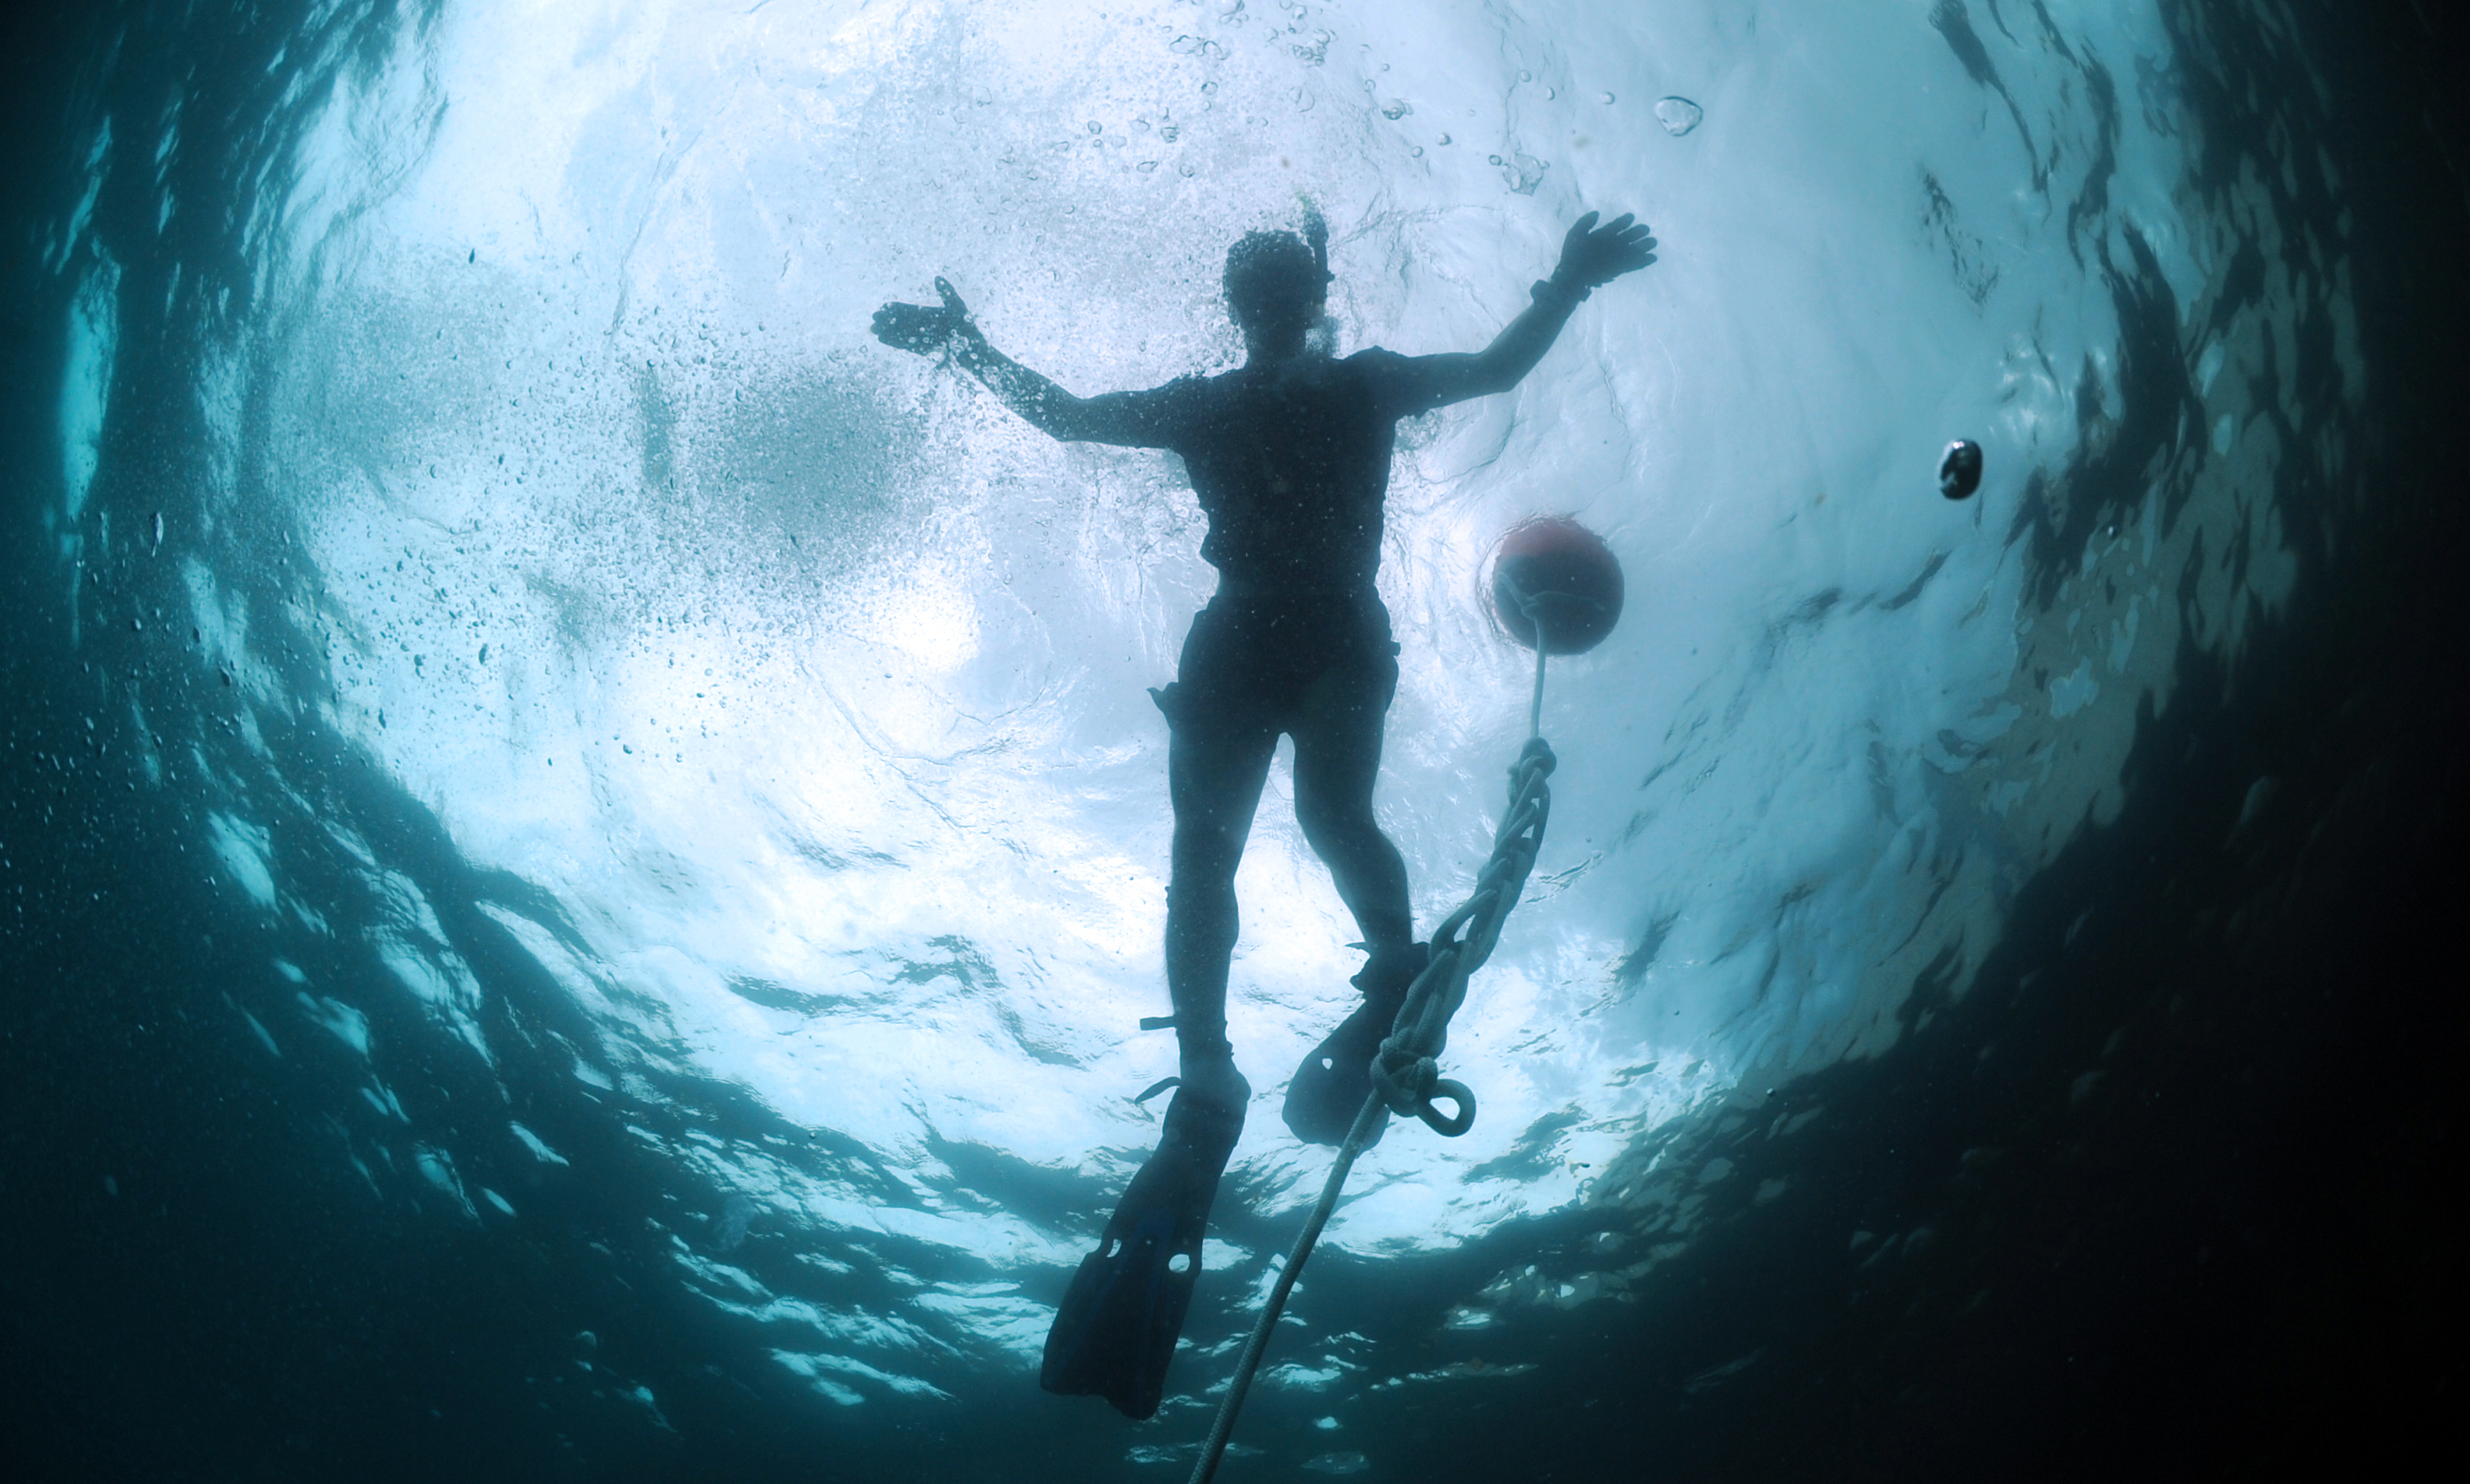
\includegraphics[scale=0.4]{snellswindow.jpg}
        \caption{Snell's window in real life. Image credit: \url{https://commons.wikimedia.org/wiki/File:US_Navy_110607-N-XD935-191_Navy_Diver_2nd_Class_Ryan_Arnold,_assigned_to_Mobile_Diving_and_Salvage_Unit_2,_snorkels_on_the_surface_to_monitor_multi.jpg} accessed on 27/04/2021.}
        \label{fig:snell's window irl}
    \end{figure}
    \begin{figure}[htbp!]
        \centering
        \tikzsetnextfilename{snells-window}
        \begin{tikzpicture}
            \fill[blue!50, opacity=0.5] (-4, -4) rectangle (4, 0);
            \draw[very thick] (0, -4) -- (-2, 0) -- (-4, 1);
            \draw[very thick] (0, -4) -- (2, 0) -- (4, 1);
            \draw[very thick] (0, -4) -- (-1.5, 0) -- (-4, 2);
            \draw[very thick] (0, -4) -- (1.5, 0) -- (4, 2);
            \draw[very thick] (0, -4) -- (-1, 0) -- (-4, 3);
            \draw[very thick] (0, -4) -- (1, 0) -- (4, 3);
            \draw[very thick] (0, -4) -- (-0.5, 0) -- (-3, 4);
            \draw[very thick] (0, -4) -- (0.5, 0) -- (3, 4);
            \draw[very thick] (0, -4) -- (0, 0) -- (0, 4);
            \draw[dashed] (-2, 0) -- (-2, -4);
            \draw[dashed] (2, 0) -- (2, -4);
        \end{tikzpicture}
        \caption{Looking up from underwater you only see out of a circle, known as Snell's window. Outside of this circle total internal reflection occurs and you see back down into the water.}
        \label{fig:snell's window}
    \end{figure}
    
    \subsubsection{Mirages}
    The refractive index of air depends on its density and hence on the temperature of the air.
    This means that on a hot day the refractive index changes a non-negligible amount between the ground and a few metres up as the air is hotter higher up.
    Imagine light coming off the top of a tree towards the ground.
    We can consider each step along the path the light takes to be going through a boundary with two different refractive indexes.
    If the conditions are just right this can cause the light to refract slightly at each step until it is travelling upwards.
    If we see this light that came from the top of a tree but is travelling upwards towards us our brains are unable to comprehend the process that has actually taken place and instead assume that the light has reflected off of something.
    Our monkey brains are also trained to see anything reflective as a source of water and therefore it is common for it to look like there is water on the ground even though there isn't.
    This is the mechanism behind heat hazes and mirages.
    
    \section{The Fresnel Equations}
    In the last section we discussed reflection and refraction with a focus on the angles that the rays make to the surface normals.
    We found that an incident ray is reflected at the same angle it is incident and that the transmitted ray will be at an angle satisfying Snell's law:
    \[n_i\sin\vartheta_i = n_t\sin\vartheta_t.\]
    To find this we solved for the wave vectors \(\vv{k_r}\) and \(\vv{k_t}\).
    We didn't however, find the amplitudes of the reflected and transmitted waves.
    This is what we will do in this section.
    To find the amplitudes we need to be slightly more cautious in our calculations and consider the direction the waves oscillate.
    There are two linearly independent directions that an incident wave can oscillate and all other cases are simply a superposition of these two cases:
    \begin{itemize}
        \item If \(\vv{E_{0i}}\) is perpendicular to the plane of incidence then we call the wave \define{transverse electric} or S-polarised\footnote{S for \textit{senkrecht}, German for perpendicular.}.
        \item If \(\vv{E_{0i}}\) is parallel to the plane of incidence then we call the wave \define{transverse magnetic} or P-polarised\footnote{P for \textit{parallel}, German for parallel.}.
    \end{itemize}
    We will treat these two cases separately.
    
    \subsection{S-Polarised Light}
    The boundary conditions for \(\vv{E}\) are that the components parallel to the boundary are continuous across the boundary.
    For S-polarised light the incoming amplitudes are perpendicular to the plane of incidence which necessarily makes them parallel to the boundary.
    Thus we must have at the boundary that
    \begin{equation}\label{eqn:continuity of electric field at boundary}
        E_{0i} + E_{0r} = E_{0t}.
    \end{equation}
    The boundary conditions are slightly more tricky for \(\vv{H}\).
    It is conventional to define \(\vv{k}\), \(\vv{E}\), and \(\vv{H}\) such that they form a right handed system.
    Considering an incoming wave being reflected the direction of \(\vv{k}\) is set by the direction of travel and the direction of \(\vv{E}\) is set by demanding S-polarised light.
    The result is that we have to choose to define the direction of \(\vv{H}\) to keep a right handed system as shown in figure~\ref{fig:S-polarised light}.
    \begin{figure}[ht]
        \centering
        \tikzsetnextfilename{reflection-transmission-amplitude-s-polarised}
        \begin{tikzpicture}
            \fill[blue!50, opacity=0.3] (-4, -4) rectangle (4, 0);
            \draw[thick] (-4, 4) -- (0, 0) -- (4, 4);
            \draw[thick] (0, 0) -- (2, -4);
            \draw[dashed] (0, 4) -- (0, -4);
            \draw[->, >=latex] (-4, 0) -- (4, 0) node[right] {\(x\)};
        
            \begin{scope}[xshift=-2cm, yshift=2cm]
                \draw[ultra thick, ->, >=latex] (0, 0) -- (-45:1) node[above right] {\(\vv{k_i}\)};
                \draw[ultra thick, ->, >=latex] (0, 0) -- (-135:1) node[left] {\(\vv{H_{0i}}\)};
                \draw[ultra thick, fill=white] (0, 0) circle[radius=0.15cm];
                \draw[fill=black] (0, 0) circle[radius=0.05cm];
                \node at (45:0.45) {\(\vv{E_{0i}}\)};
            \end{scope}
        
            \begin{scope}[xshift=2cm, yshift=2cm]
                \draw[ultra thick, ->, >=latex] (0, 0) -- (45:1) node[above left] {\(\vv{k_r}\)};
                \draw[ultra thick, ->, >=latex] (0, 0) -- (-45:1) node[right] {\(\vv{H_{0r}}\)};
                \draw[ultra thick, fill=white] (0, 0) circle[radius=0.15cm];
                \draw[fill=black] (0, 0) circle[radius=0.05cm];
                \node at (135:0.45) {\(\vv{E_{0r}}\)};
            \end{scope}
        
            \begin{scope}[xshift=1cm, yshift=-2cm]
                \draw[ultra thick, ->, >=latex] (0, 0) -- ({atan(1/2)-90}:1) node[above right] {\(\vv{k_i}\)};
                \draw[ultra thick, ->, >=latex] (0, 0) -- ({atan(1/2)+180}:1) node[left] {\(\vv{H_i}\)};
                \draw[ultra thick, fill=white] (0, 0) circle[radius=0.15cm];
                \draw[ultra thick, fill=blue!50, fill opacity=0.3] (0, 0) circle[radius=0.15cm];
                \draw[fill=black] (0, 0) circle[radius=0.05cm];
                \node at ({atan(1/2)}:0.45) {\(\vv{E_i}\)};
            \end{scope}
        
            \begin{scope}
                \clip (0, 0) -- (-4, 4) -- (0, 4) -- cycle;
                \draw (0, 0) circle[radius=0.5cm];
            \end{scope}
            \begin{scope}
                \clip (0, 0) -- (4, 4) -- (0, 4) -- cycle;
                \draw (0, 0) circle[radius=0.75cm];
            \end{scope}
            \begin{scope}
                \clip (0, 0) -- (2, -4) -- (0, -4) -- cycle;
                \draw (0, 0) circle[radius=0.5cm];
            \end{scope}
            \node at (112:0.7) {\(\vartheta_i\)};
            \node at (62:0.9) {\(\vartheta_r\)};
            \node at ({-90+atan(1/2)/2}:0.7) {\(\vartheta_t\)};
        \end{tikzpicture}
        \caption{S-polarised light reflection and transmission.}
        \label{fig:S-polarised light}
    \end{figure}
    In particular we have \(\vv{k}\times\vv{E} = v\vv{B}\).
    We can then show that the continuity equation for \(\vv{H}\) is
    \[H_{0i}\cos\vartheta_i - H_{0r}\cos\vartheta_r = H_{0t}\cos\vartheta_t.\]
    Writing \(H = B/\mu = E/(v\mu) = En/(c\mu)\) and \(\vartheta_r = \vartheta_i\) we have
    \begin{align*}
        \frac{B_{0i}}{\mu_i}\cos\vartheta_i - \frac{B_{0r}}{\mu_i}\cos\vartheta_i &= \frac{B_{0t}}{\mu_t}\cos\vartheta_t\\
        \frac{E_{0i}n_i}{c\mu_i}\cos\vartheta_i - \frac{E_{0r}n_i}{c\mu_i}\cos\vartheta_i &= \frac{E_{0t}n_t}{c\mu_t}\cos\vartheta_t\\
        (E_{0i} - E_{0r})\frac{n_i\cos\vartheta_i}{c\mu_i} = E_{0t}\frac{n_t\cos\vartheta_t}{c\mu_t} &= (E_{0i} + E_{0r})\frac{n_t\cos\vartheta_t}{c\mu_t}
    \end{align*}
    where in the last equality we have used the continuity equation for the electric field (equation~\ref{eqn:continuity of electric field at boundary}).
    Since we can link \(\vartheta_i\) and \(\vartheta_t\) by Snell's law and we can measure the material properties \(\mu_i\), \(\mu_t\), \(n_i\), and \(n_t\) this equation gives us a relationship between the amplitudes of the incident magnetic field, \(E_{0i}\), and the reflected field, \(E_{0r}\).
    
    We further assume that the magnetic field is not that strong and so it is a reasonable approximation to assume that \(\mu_i = \mu_t = \mu_0\).
    We define the \define{Fresnel reflection coefficient} as the ratio \(E_{0r}/E_{0i}\) which for S-polarised light we find to be
    \[\fresnelCoeff{r}{S} = \frac{E_{0r}}{E_{0i}} = \frac{n_i\cos\vartheta_{i} - n_t\cos\vartheta_{t}}{n_i\cos\vartheta_i + n_t\cos\vartheta_t}.\]
    We can use the same equations and instead eliminate \(E_{0r}\) leaving us with a relationship between \(E_{0t}\) and \(E_{0i}\).
    Similarly we can then define the \define{Fresnel trnasmission coefficeint} for S-polarised light:
    \[\fresnelCoeff{t}{S} = \frac{E_{0t}}{E_{0i}} = \frac{2n_{i}\cos\vartheta_{i}}{n_i\cos\vartheta_{i} + n_t\cos\vartheta_{t}}.\]
    
    \subsection{P-Polarised Light}
    The case of P-polarised light is very similar with slightly different boundary conditions.
    This time the \(\vv{H}\) continuity equation is simple:
    \[H_{0i} + H_{0r} = H_{0t}\]
    and the \(\vv{E}\) continuity equations are the more complicated
    \[E_{0i}\cos\vartheta_i - E_{0r}\cos\vartheta_i = E_{0t}\cos\vartheta_t.\]
    We can similarly define \define{Fresnel coefficients} for reflection and transmission of P-polarised light:
    \begin{align*}
        \fresnelCoeff{r}{P} &= \frac{E_{0r}}{E_{0i}} = \frac{n_t\cos\vartheta_i - n_i\cos\vartheta_t}{n_i\cos\vartheta_t + n_t\cos\vartheta_i},\\
        \fresnelCoeff{t}{P} &= \frac{E_{0t}}{E_{0i}} = \frac{2n_i\cos\vartheta_i}{n_i\cos\vartheta_t + n_t\cos\vartheta_i}.\\
    \end{align*}
    \begin{figure}[ht]
        \centering
        \tikzsetnextfilename{reflection-transmission-amplitude-p-polarised}
        \begin{tikzpicture}
            \fill[blue!50, opacity=0.3] (-4, -4) rectangle (4, 0);
            \draw[thick] (-4, 4) -- (0, 0) -- (4, 4);
            \draw[thick] (0, 0) -- (2, -4);
            \draw[dashed] (0, 4) -- (0, -4);
            \draw[->, >=latex] (-4, 0) -- (4, 0) node[right] {\(x\)};
            
            \begin{scope}[xshift=-2cm, yshift=2cm]
                \draw[ultra thick, ->, >=latex] (0, 0) -- (-45:1) node[above right] {\(\vv{k_i}\)};
                \draw[ultra thick, ->, >=latex] (0, 0) -- (45:1) node[right] {\(\vv{E_{0i}}\)};
                \draw[ultra thick, fill=white] (0, 0) circle[radius=0.15cm];
                \draw[fill=black] (0, 0) circle[radius=0.05cm];
                \node at (-135:0.45) {\(\vv{H_{0i}}\)};
            \end{scope}
            
            \begin{scope}[xshift=2cm, yshift=2cm]
                \draw[ultra thick, ->, >=latex] (0, 0) -- (45:1) node[right] {\(\vv{k_r}\)};
                \draw[ultra thick, ->, >=latex] (0, 0) -- (135:1) node[left] {\(\vv{E_{0r}}\)};
                \draw[ultra thick, fill=white] (0, 0) circle[radius=0.15cm];
                \draw[fill=black] (0, 0) circle[radius=0.05cm];
                \node at (-45:0.5) {\(\vv{H_{0r}}\)};
            \end{scope}
            
            \begin{scope}[xshift=1cm, yshift=-2cm]
                \draw[ultra thick, ->, >=latex] (0, 0) -- ({atan(1/2)-90}:1) node[above right] {\(\vv{k_i}\)};
                \draw[ultra thick, ->, >=latex] (0, 0) -- ({atan(1/2)}:1) node[right] {\(\vv{E_i}\)};
                \draw[ultra thick, fill=white] (0, 0) circle[radius=0.15cm];
                \draw[ultra thick, fill=blue!50, fill opacity=0.3] (0, 0) circle[radius=0.15cm];
                \draw[fill=black] (0, 0) circle[radius=0.05cm];
                \node at ({180+atan(1/2)}:0.45) {\(\vv{H_i}\)};
            \end{scope}
            
            \begin{scope}
                \clip (0, 0) -- (-4, 4) -- (0, 4) -- cycle;
                \draw (0, 0) circle[radius=0.5cm];
            \end{scope}
            \begin{scope}
                \clip (0, 0) -- (4, 4) -- (0, 4) -- cycle;
                \draw (0, 0) circle[radius=0.75cm];
            \end{scope}
            \begin{scope}
                \clip (0, 0) -- (2, -4) -- (0, -4) -- cycle;
                \draw (0, 0) circle[radius=0.5cm];
            \end{scope}
            \node at (112:0.7) {\(\vartheta_i\)};
            \node at (62:0.9) {\(\vartheta_r\)};
            \node at ({-90+atan(1/2)/2}:0.7) {\(\vartheta_t\)};
        \end{tikzpicture}
        \caption{P-polarised light reflection and transmission.}
    \end{figure}

    \subsection{Fresnel Coefficients With Incidence Angle}
    Consider light incident on glass (\(n = 1.5\)) travelling from air (\(n = 1\)).
    For normal, or almost normal incidence (\(\vartheta_i \approx 0\)) we see that for both S and P-polarised light we have \(\abs{t} \gg \abs{r}\).
    Comparing this to our daily experiences this makes sense as we are used to light passing straight through glass.
    For grazing incidence (\(\vartheta_i \approx \pi/2\)) we see that \(\abs{t} \approx 0\) and \(\abs{r} \approx 1\).
    Again this should be familiar that glass viewed at a large incidence angle is almost entirely reflective.
    
    For all angles of incidence it turns out that \(\fresnelCoeff{r}{S} < 0\).
    This corresponds to the incident and reflected \(\vv{E}\) fields being antiparallel.
    That is S-polarised light undergoes a phase shift of \(\pi\) when reflecting off of a higher refractive index medium.
    
    For P-polarised light at some point \(\fresnelCoeff{r}{P}\) becomes zero.
    The angle, \(\brewstersAngle\), at which this occurs is called \define{Brewster's angle}.
    At this angle there is no reflection.
    
    The transmission coefficients are similar (but not identical, note the refractive indices in the denominator swap) for both S and P-polarised light.
    It is mostly in reflection where the polarisation is important.
    
    Now consider the opposite case of light incident on a glass-air boundary from within the glass.
    For near normal incidence almost all light is transmitted.
    For P-polarised light there is an angle at which no light is reflected.
    This is sometimes referred to as the \define{internal Brewster's angle}.
    Note that this angle is \emph{not} the same angle as for the air-glass boundary.
    
    There is no phase shift for reflection of S-polarised light (as opposed to the \(\pi\) phase shift for the air-glass case).
    
    Above some critical angle, \(\criticalAngle\), both \(\fresnelCoeff{r}{S}\) and \(\fresnelCoeff{r}{P}\) are 1 and \(\fresnelCoeff{t}{S}\) and \(\fresnelCoeff{t}{P}\) are 0.
    This corresponds to total internal reflection.
    
    Perhaps the seemingly weirdest thing is that \(t > 1\) which means that, even if some light is reflected, the incident electric field has a smaller amplitude than the transmitted electric field.
    We will see in the next section why this must be the case.
    
    \subsection{Energy Flow}
    The amplitude of the transmitted field being greater than the amplitude of the incident field initially seems to violate energy conservation.
    As is often the case in electromagnetism this is because energy scales with the \emph{square} of the amplitude.
    For an oscillating field the most useful quantity is the intensity, \(I\), defined as the time average of the magnitude of the Poynting vector, \(\vv{S}\):
    \[I = \expected{S} = \frac{v\varepsilon}{2}E_0^2.\]
    Here \(v = c/n\) and we replace \(\varepsilon_0\) with \(\varepsilon\) when inside a medium.
    This gives the power density per unit area normal to the Poynting vector.
    
    Suppose we illuminate an area, \(A\), on a surface.
    To conserve energy we have to have the energy in per unit time be equal to the energy out per unit time.
    That is
    \[I_iA\cos\vartheta_i = I_rA\cos\vartheta_r + I_tA\cos\vartheta_t\]
    where \(I_i\), \(I_r\), and \(I_t\) are the intensities of the incident, reflected, and transmitted, field respectively.
    We can rearrange this and use the fact that \(\vartheta_i = \vartheta_r\) to get
    \[\frac{I_r}{I_i} + \frac{I_t}{I_i} \frac{\cos\vartheta_t}{\cos\vartheta_i} = 1.\]
    The first term gives the fraction of incident energy that is reflected and the second gives the fraction of incident energy that is transmitted.
    We call the first fraction the \define{reflectivity}:
    \[R = \frac{I_r}{I_i} = \frac{E_{0r}^2}{E_{0i}^2} = r^2.\]
    The second term we call the \define{transmissivity}:
    \[T = \frac{I_t}{I_i}\frac{\cos\vartheta_t}{\cos\vartheta_i} = \frac{E_{0t}^2}{E_{0i}^2} \frac{\mu_{ri}^2}{\mu_{rt}^2}\frac{n_t}{n_i}\frac{\cos\vartheta_t}{\cos\vartheta_i} \approx \frac{E_{0t}^2}{E_{0i}^2}\frac{n_t}{n_i}\frac{\cos\vartheta_t}{\cos\vartheta_i} = t^2\frac{n_t}{n_i}\frac{\cos\vartheta_t}{\cos\vartheta_i}.\]
    It can be shown that \(R + T = 1\) for all incident angle and this is the condition that energy is conserved.
    This explains why we can have \(t > 1\) so long as \(r\) is such that \(R +  T = 1\).
    
    At normal incidence for an air-glass boundary \SI{4}{\percent} of the light is reflected.
    For a single boundary this is negligible and we treat it as pure transmission.
    The issue arises with multiple boundaries, such as in a telescope or microscope, where there are multiple lenses and therefore the light we get out will be of significantly lower intensity than the light that we put in.
    The way that the unwanted reflected beams affect the image we get out is also non-trivial.
    
    So far in this section we have assumed that no energy is absorbed by the medium.
    If this isn't the case then the quantities \(r\), \(t\), \(n\), and \(\varepsilon\) become complex.
    We will see this more later.
    
    For a glass-air boundary above the critical angle \(R\) becomes 1 and \(T\) becomes 0.
    This is due to total internal reflection.
    
    \section{Consequences of the Fresnel Equations}
    \subsection{Total Internal Reflection}
    In the calculation of the Fresnel coefficients the transmission angle, \(\vartheta_t\), appears explicitly.
    The problem is that we can't define \(\vartheta_t\) for incidence angles greater than the critical angle.
    The way we solve this is by using Snell's law and trig identities:
    \[
        \left.
        \begin{array}{r}
        n_i\sin\vartheta_i = n_t\sin\vartheta_t \implies \sin\vartheta_t =  \frac{n_i}{n_t}\sin\vartheta_i\\
        \\
        \sin^2\vartheta_t + \cos^2\vartheta_t \implies \cos\vartheta_t = \sqrt{1 - \sin^2\vartheta_t}
        \end{array}
        \right\} \implies
        \cos\vartheta_t = \sqrt{1 - \frac{n_i^2}{n_t^2} \sin^2\vartheta_i}.
    \]
    Using this we can write the reflection coefficient as
    \[\fresnelCoeff{r}{S} = \frac{\cos\vartheta_i - \sqrt{n_t^2/n_i^2 - \sin^2\vartheta_i}}{\cos\vartheta_i + \sqrt{n_t^2/n_i^2 - \sin^2\vartheta_i}}.\]
    For cases where we have total internal reflection we have \(n_t/n_i < \sin\vartheta_i\) which means that the square roots result in complex numbers.
    We can generalise the reflectivity and transmissivity from the last section.
    In doing so we have to treat the S and P-polarised cases differently:
    \[\fresnelCoeff{R}{S} = \fresnelCoeff{r}{S}^*\fresnelCoeff{r}{S}, \qquad\text{and}\qquad \fresnelCoeff{R}{P} = \fresnelCoeff{r}{P}^*\fresnelCoeff{r}{P}.\]
    It can be shown that both reflectivities become 1 above the critical angle.
    
    When total internal reflection occurs the transmitted field has intensity 0.
    However in order for the correct continuity rules to apply we need to have a wave still.
    It can be shown that the if the transmitted wave vector is \(\vv{k_t}\) then the component parallel to the boundary is \(k_t\sin\vartheta_t\) which can be expressed as \(k_t(n_i/n_t)\sin\vartheta_i\) using Snell's law.
    The component perpendicular to the boundary can be expressed as
    \[k_t\cos\vartheta = k_t\sqrt{1 - \frac{n_i^2}{n_t^2}\sin^2\vartheta_i}.\]
    For total internal reflection we can write this as \(\pm i\beta\).
    This imaginary component to the wave vector corresponds to exponential decay of this component of the \(\vv{E}\) field.
    So for total internal reflection the transmitted ray decays to zero.
    These are called \define{evanescent} or \define{boundary waves}.
    If we make the low refractive index layer very thin then it is possible to get the transmitted wave out the other side before it decays to zero.
    This is called \define{frustrated total internal reflection}.
    
    \subsection{Metals and Plasmas}
    We saw something similar to evanescent waves when we considered electromagnetic fields incident on metal.
    We saw that the fields penetrate only a small amount, called the skin depth.
    
    Equation~\ref{eqn:epsilon r oscillator model} gives the relative permittivity derived from the oscillator model.
    If we allow for free electrons as well then we get instead
    \[\varepsilon_r = \varepsilon_r' + i\varepsilon_r'' = 1 + \frac{N\chargeElectron^2}{\varepsilon_0\massElectron} \left[ \frac{f_{\mathrm{e}}}{-\omega^2 - i\gamma_{\mathrm{e}}} + \sum_{j} \frac{f_j}{\omega_{0j}^2 - \omega^2 - i\gamma_j\omega} \right]\]
    The second term corresponds to the bound electrons summing over all relevant natural frequencies and the first term is the same but for unbound electrons so \(\omega_0 = 0\).
    The numerators, \(f_{\mathrm{e}}\) and \(f_j\) give the fraction of electrons that fall into each of these categories.
    
    The addition of the extra term changes the optical behaviour of the materials.
    For transparent dielectrics, such as glass, the natural frequency is \(\omega_0 \sim \SI{e16}{\radian.s^{-1}}\), which corresponds to the UV part of the spectrum.
    This means that visible light has \(\omega < \omega_0\) which we saw corresponds to the electron cloud oscillating \(\pi\) out of phase with \(\vv{E}\) and so the dipoles oscillate in phase with \(\vv{E}\).
    For free electrons the frequency of the driving force is above \(\omega_0\), even for visible light, which means that the oscillating electrons radiate wavelets that cancel the incident wave.
    
    Ignoring the bound electron's contribution and neglecting damping, \(\gamma_{\mathrm{e}} = 0\), the relative permittivity is given by
    \[\varepsilon_r = 1 - \frac{N\chargeElectron^2}{\varepsilon_0\massElectron\omega^2} = 1 - \frac{\omega_p^2}{\omega^2}\]
    where this equation defines \(\omega_p\), called the \define{plasma frequency}.
    For \(\omega < \omega_p\) we have \(\varepsilon_r < 0\) and hence the refractive index is imaginary, \(n = i\sqrt{\omega_p^2/\omega^2 - 1}\).
    The reflectivity at normal incidence can then be shown to be 1.
    If instead \(\omega > \omega_p\) then \(\varepsilon_r > 0\) and \(n = \sqrt{1 - \omega_p^2/\omega^2} \in\reals\).
    The reflectivity falls rapidly to zero as \(\omega\) increases.

    While these results only apply exactly for free electrons (a plasma) lots of metals can be reasonably approximated as a plasma of free electrons and some bound electrons and these results still approximately apply.
    This means that metals are transparent to light with \(\omega > \omega_p\).
    For most metals \(\omega_p\) is in the deep-UV part of the spectrum.
    
    The upper atmosphere is subject to intense solar radiation and is therefore highly ionised.
    Calculating \(\omega_p\) based on the charge density of the ionosphere we predict \(\omega_p\) to be in the \si{\mega\hertz} range meaning that lower frequency electromagnetic waves should be reflected back down to Earth.
    This is indeed the case and we use it to send radio messages from one place to another without direct line of site.
    
    \part{Superposition}
    \section{Superposition of Waves with the Same Wave Vector}
    So far we have only considered one wave at a time.
    If we want to consider more complicated phenomena such as multiple reflections or interference we need a solid mathematical understanding of what happens when two waves occupy the same region of space.
    We need superposition.
    
    The simplest case is two waves with the same wave vector and frequency.
    These waves differ only in their amplitude, \(E_{0i}\), and phase, \(\Phi_{i}\).
    For simplicity we define our coordinate system such that the common wave vector, \(k\), is aligned with the \(z\)-axis.
    Then each wave has the functional form
    \[E_{i} = E_{0i}\cos(kz - \omega t - \Phi_i).\]
    The resulting field then has amplitude \(E = E_{1} + E_{2}\) given by
    \begin{align*}
        E &= E_{01}\cos(kz - \omega t - \Phi_1) + E_{02}\cos(kz - \omega t - \Phi_2)\\
        &= E_{01}[\cos(kz - \omega t)\cos\Phi_1 + \sin(kz - \omega t) \sin\Phi_1] + E_{02}[\cos(kz - \omega t)\cos\Phi_2 + \sin(kz - \omega t)\sin\Phi_2]\\
        &= [E_{01}\cos\Phi_1 + E_{02}\cos\Phi_2]\cos(kz - \omega t) + [E_{01}\sin\Phi_1 + E_{02}\sin\Phi_2]\sin(kz - \omega t).
    \end{align*}
    So we see that the resultant field, \(E\), is also a harmonic wave,
    \[E = E_{0}\cos(kz - \omega t - \Phi)\]
    where
    \[E_{0}\cos\Phi = E_{01}\cos\Phi_1 + E_{02}\cos\Phi_2, \qquad\text{and}\qquad E_{0}\sin\Phi = E_{01}\sin\Phi_1 + E_{02}\sin\Phi_2\]
    which can be achieved by setting
    \begin{equation}\label{eqn:E0 and Phi}
        E_{0}^2 = E_{01}^2 + E_{02}^2 + 2E_{01}E_{02}\cos(\Phi_1 - \Phi_2), \qquad\text{and}\qquad \Phi = \arctan\left[ \frac{E_{01}\sin\Phi_1 + E_{02}\sin\Phi_2}{E_{01}\cos\Phi_1 + E_{02}\cos\Phi_2} \right].
    \end{equation}
    See figure~\ref{fig:superposition same k and omega}.
    
    \begin{figure}[ht]
        \centering
        \tikzsetnextfilename{superposition-same-k-and-omega}
        \begin{tikzpicture}
            \begin{axis}[
                xlabel=\(z\),
                domain=0:20,
                ymin=-2.2,
                ymax=2.2,
                samples=200
            ]
                \addplot[color=blue, thick] {1.2*cos(deg(x))};
                \addlegendentry{\(E_1\)}
                \addplot[color=red, thick] {0.8*cos(deg(x - 1))};
                \addlegendentry{\(E_2\)}
                \addplot[color=red!50!blue, thick] {1.2*cos(deg(x)) + 0.8*cos(deg(x - 1))};
                \addlegendentry{\(E\)}
            \end{axis}
        \end{tikzpicture}
        \caption{A snapshot at some fixed time \(t\) showing two harmonic waves, \(E_i\), with the same wave vector but different amplitudes and phases and their superposition, \(E\). Notice that \(E\) is a harmonic wave.}
        \label{fig:superposition same k and omega}
    \end{figure}

    Now that we have seen the superposition of two harmonic waves with the same frequency and wave vector the superposition of \(N\) harmonic waves all with the same frequency and wave vector is simply given by
    \[E = \sum_{i=1}^{N} E_{0i}\cos(kz - \omega t - \Phi_{i}) = E_0\cos(kz - \omega t - \Phi).\]
    
    \subsection{Alternative Computations}
    We computed the superposition using lots of trig identities.
    This is perhaps the slowest and least enlightening way to compute superpositions.
    The most efficient way is probably using complex exponentials and simply discarding the imaginary part when we need the actual physical wave.
    The starting waves are then given by
    \[E_i = E_{0i}\exp[i(kz - \omega t - \Phi_i)] = E_{01}\exp(-i\Phi_i)\exp[i(kz - \omega t)].\]
    The superposition of two waves is then
    \[E = E_1 + E_2 = E_0\exp(-i\Phi)\exp[i(kz - \omega t)]\]
    where \(E_0\) and \(\Phi\) are given in equation~\ref{eqn:E0 and Phi}.
    
    The same computation can also be done graphically with phasors which are simply vectors in the complex plane (viewed as a two dimensional real vector space) and we then simply perform normal vector addition to get the amplitude and phase which are simply the magnitude and angle of the resulting vector.
    See figure~\ref{fig:phasor addition}
    \begin{figure}[ht]
        \centering
        \tikzsetnextfilename{phasor-addition}
        \begin{tikzpicture}
            \tikzset{vector/.style={ultra thick, ->, >=latex}}
            \draw[vector] (0, 0) -- (2, -1) node[pos=0.75, above] {\(E_{01}\)};
            \draw[vector] (2, -1) -- (3, -3) node[midway, right] {\(E_{02}\)};
            \draw[vector] (0, 0) -- (3, -3) node[midway, below left] {\(E\)};
            \draw[dashed] (0, 0) -- (2, 0);
            \draw[dashed] (2, -1) -- (3, -1);
            \begin{scope}
                \clip (0, 0) -- (2, -1) -- (2, 0) -- cycle;
                \draw (0, 0) circle[radius=0.8cm];
            \end{scope}
            \begin{scope}
                \clip (2, -1) -- (3, -3) -- (3, -1) -- cycle;
                \draw (2, -1) circle[radius=0.5cm];
            \end{scope}
            \begin{scope}
                \clip (0, 0) -- (3, -3) -- (3, 0);
                \draw (0, 0) circle[radius=0.6cm];
            \end{scope}
            \node at (-12:1.1) {\(\Phi_1\)};
            \begin{scope}[xshift=2cm, yshift=-1cm]
                \node at (-30:0.8) {\(\Phi_2\)};
            \end{scope}
            \node at (-36:1.1) {\(\Phi\)};
        \end{tikzpicture}
        \caption{Addition of two phasors.}
        \label{fig:phasor addition}
    \end{figure}
    
    \subsection{Intensities}
    The intensity of the field is proportional to the amplitude squared.
    In fact \(I = v\varepsilon E_0^2/2\) however it is common to just work with \(I = E_0^2\) when we only want to compare intensities within a single medium.
    From equation~\ref{eqn:E0 and Phi} we see that
    \[E_0^2 = E_{01}^2 + E_{02}^2 + 2E_{01}E_{02}^2\cos(\Phi_{1} - \Phi_{2}).\]
    So the total intensity is the sum of the intensities plus an interference term which may be positive or negative depending on how in phase the waves are.
    
    The maximum (resp. minimum) intensity is achieved when the phase difference \(\Phi_1 - \Phi_2\) is an even (resp. odd) multiple of \(\pi\) and we have
    \[E_{0}^2{_{\min\mkern-4mu/\mkern-4mu\max}} = E_{01}^2 + E_{02}^2 \pm 2E_{01}E_{02} = (E_{01} \pm E_{02})^2.\]
    So for the special case of \(E_{01} = E_{02}\) it is possible that the intensity of the resulting wave will be anywhere from 0 to \(4E_{01}\).
    
    \subsection{Phases}
    There are a few mechanisms by which a phase difference can appear:
    \begin{itemize}
        \item The first crests of the two waves leave the emitters at different times by a non-integer multiple of the period.
        \item The two emitters are a non-integer number of wavelengths apart.
        \item The two waves start in phase but then one passes through a more optically dense material.
    \end{itemize}
    To be rigorous about the third of these we introduce the idea of an \define{phase thickness} which is defined to be
    \[\delta = \frac{2\pi d}{\lambda}\]
    where \(d\) is the actual thickness of the material and \(\lambda\) is the wavelength of the light in the medium.
    In terms of the vacuum wavelength, \(\lambda_0\), we have
    \[\delta = \frac{2\pi nd}{\lambda_0}.\]
    This quantity is related to the optical thickness, \(nd\), but the phase thickness accounts for the phase difference between light that travels through the medium and the same light if it had been unimpeded.
    If the difference in phase thickness is caused purely by a difference in refractive indices then it is sometimes referred to as \define{retardation}.
    
    \subsection{Coherence}
    We have so far assumed that the phase difference, \(\Phi_1 - \Phi_2\), is constant.
    We will see later that this isn't always the case and we will introduce notions of coherence time and coherence length which are scales over which the phase difference is approximately constant.
    
    \section{More Superposition}
    \subsection{Standing Waves}
    Suppose two waves of the same frequency, \(\omega\), are travelling in opposite directions with different amplitudes.
    The resultant field has amplitude
    \[E(z, t) = E_{0L}\cos(kz - \omega t) + E_{0R}\cos(kz + \omega t).\]
    If \(E_{0L} = E_{0R}\) then some basic trig identities lead us to conclude that
    \[E(z, t) = 2E_{0L}\cos(kz)\cos(\omega t).\]
    This is different to waves we have studied so far in that it is not of the form \(f(z \pm vt)\) or \(f(kz \pm \omega t)\).
    Instead we have oscillations based on position, \(z\), and oscillations with time, \(t\).
    All points in the wave rise and fall at the same time.
    This is a \define{standing wave}.
    
    It can be shown that for a standing wave the magnetic field is
    \[B(z, t) = \frac{E(z', t')}{c}\]
    where \(z' = z - \lambda/4\) and \(t' = t - T/4\) which corresponds to \(\vv{B}\) and \(\vv{E}\) being perpendicular but put of phase by \(\pi/2\).
    An important quantity for standing waves is the Poynting vector, \(\vv{S} = \vv{E}\times\vv{B}\).
    This calculation is complicated by the fact that \(\vv{B} \ne \vv{E}/c\) which we have relied on in the past.
    It can be shown that
    \[\vv{S} = c\varepsilon_0E_0^2 \sin(2kz)\sin(2\omega t)\ve{z}.\]
    So \(\vv{S}\) is always along the \(z\) direction but its amplitude and sign oscillate in time and space in such a way that
    \[I = \expected{S} = 0.\]
    So for a standing wave there is no flow of energy.
    There is movement of energy but it moves forward and back so the net result is no energy flow.
    
    \subsection{Superposition with Similar Frequencies}
    Consider two waves that are \emph{almost} the same.
    For example these waves may be produced by the same source and have the same amplitude, \(E_{01}\), but slightly different wave vectors and frequencies.
    These waves are given by
    \[E_1 = E_{01}\cos(k_iz - \omega_i t).\]
    We can use the trig identity
    \[\cos\alpha + \cos\beta = 2 \cos\left( \frac{1}{2}(\alpha + \beta) \right)\cos\left( \frac{1}{2}(\alpha - \beta) \right).\]
    The superposition of these waves is then
    \[E = 2E_{01} \cos\left[ \left( \frac{k_1 + k_2}{2}z - \left( \frac{\omega_1 - \omega_2}{2} \right) \right) \right] \cos\left[ \left( \frac{k_1 - k_2}{2} \right)z - \left( \frac{\omega_1 - \omega_2}{2} \right)t \right].\]
    Notice that this appears to be the product of two different waves.
    We call the first the \define{carrier} wave and it has frequency and wave vector
    \[\omega_c = \frac{\omega_1 + \omega_2}{2}, \qquad\text{and}\qquad k_c = \frac{k_1 + k_2}{2}.\]
    The second is called the \define{modulation} wave and it has frequency and wave vector
    \[\omega_m = \frac{\omega_1 - \omega_2}{2}, \qquad\text{and}\qquad k_m = \frac{k_1 - k_2}{2}.\]
    So the resulting wave is
    \[E = 2E_{01}\cos(k_cz - \omega_ct)\cos(k_mz - \omega_t).\]
    Since \(\omega_1 \approx \omega_2\) and \(k_1 \approx k_2\) we have that \(\omega_c \gg \omega_m\) and \(k_c \gg k_m\).
    The result is a wave with approximate frequency and wave vector \(\omega_c\) and \(k_c\) which is attenuated by a wave with frequency \(\omega_m\) and wave vector \(k_m\).
    This can be seen in figure~\ref{fig:carrier and modulating wave}.
    
    \begin{figure}[htp]
        \centering
        \tikzsetnextfilename{superposition-carrier-and-modulating-wave}
        \begin{tikzpicture}
            \begin{axis}[
                domain=0:20,
                xlabel=z,
                samples=800,
                width=15cm
            ]
                \addplot[thick, red, dashed] {cos(deg(6*x))};
                \addlegendentry{Carrier Wave}
                \addplot[thick, blue, dashed] {2*cos(deg(x))};
                \addlegendentry{Modulating Wave}
                \addplot[very thick, red!50!blue] {2*cos(deg(6*x))*cos(deg(x))};
                \addlegendentry{Superposition}
            \end{axis}
        \end{tikzpicture}
        \caption{The superposition of two waves with similar frequency and wave vector results in a carrier wave attenuated by a lower frequency wave.}
        \label{fig:carrier and modulating wave}
    \end{figure}
    The intensity of this wave is found by averaging \(\abs{\vv{S}}\) over one period of the carrier wave.
    This gives
    \[I \propto 4E_{01}^2\cos^2(k_mz - \omega_mt) = 2E_{01}^2[1 + \cos(2(k_mz - \omega_mt))].\]
    We see that the intensity varies from 0 to \(4E_{01}^2\) with frequency \(2\omega_{m}\), which is known as the beats frequency.
    We can actually hear the beats frequency if we choose two notes close in frequency but differing by a few hertz.
    
    \subsubsection{Group and Phase Velocity}
    The dispersion of electromagnetic waves in media leads to different phase velocities at different frequencies.
    Notice we introduce the modifier here `phase' as we will see there is a second velocity of interest in this scenario.
    
    The modulation wave moves with velocity \(v_m\) given by the dispersion relationship:
    \[v_m = \frac{\omega_m}{k_m} = \frac{\omega_1 - \omega_2}{k_1 - k_2} = \frac{\Delta \omega}{\Delta k}.\]
    Assuming that \(\omega_c \gg \omega_m\), i.e. that \(\omega_1 \approx \omega_2\) and similarly \(k_c \gg k_m\) this ratio of differences can be approximated with a derivative:
    \[v_g = \dv{\omega}{k}\]
    where \(v_g\) is known as the \define{group velocity} and is the velocity of the envelope (modulation wave).
    We can relate the group velocity and the phase velocity (which up until this point we have simply referred to as velocity) by noting that \(\omega = ck/n\) and also refractive index depends on frequency so \(n = n(\omega)\) which means that
    \[\omega = \frac{ck}{n(\omega)} = v_p(\omega)k.\]
    Differentiating this and rearranging we get
    \[v_g = \dv{\omega}{k} = \frac{1}{n + \omega \inlinedv{n}{\omega}} = \frac{v_p}{1 - (\omega/v_p)\inlinedv{v_p}{\omega}}.\]
    One interesting consideration here is that it is possible that \(v_p\) can be greater than \(c\).
    This seems to disagree with special relativity but it turns out that no information can be transmitted at the phase velocity, the only way information can be sent in this case is in the resulting wave which travels at the group velocity, which is always lower than \(c\).
    So special relativity isn't violated.
    
    \section{Fourier Analysis}
    Up until now in this part we have taken two (or more) waves and computed the resulting field.
    In this section we will look at the resulting wave and attempt to recover the individual waves.
    Assuming that the only waves present are harmonic we can do this using Fourier analysis.
    
    
    Consider some periodic wave, \(f\), which is not necessarily harmonic.
    By periodic we mean there exists some \(\lambda\in\reals\) such that \(f(z) = f(z + \lambda)\).
    Then we can decompose \(f\) (under some fairly week conditions) as
    \[f(z) = \frac{A_0}{2} + \sum_{m=1}^{\infty} A_m\cos(mkz) + \sum_{m=1}^{\infty} \sin(mkz)\]
    where \(k = 2\pi/\lambda\), and \(A_m\) and \(B_m\) are real constants given by
    \[A_m = \frac{2}{\lambda} \int_{0}^{\lambda} f(z) \cos(mkz)\dd{z}, \qquad\text{and}\qquad B_m = \frac{2}{\lambda}\int_{0}^{\lambda} f(z)\sin(mkz)\dd{z}.\]
    
    For a non-periodic wave we can consider it to be a periodic function which repeats at infinity.
    A proper limiting process\footnote{See the Fourier analysis part of the Fourier analysis and statistics course} gives us
    \[f(z) = \frac{1}{\pi} \left[ \int_{0}^{\infty} A(k)\cos(kz)\dd{k} + \int_{0}^{\infty} B(k)\sin(kz)\dd{k} \right]\]
    where \(A\) and \(B\) are now functions of \(k\in\reals\)
    
    \begin{example}
        Consider the function \(f\), defined by
        \[
            f(z) =
            \begin{cases}
                1/L, & \text{if}~z\in[-L/2, L/2],\\
                0, & \text{else}.
            \end{cases}
        \]
        The Fourier transform of this is
        \begin{align*}
            \hat{f}(k) &= \FT[f](k) \\
            &= \int_{-\infty}^{\infty} f(z)e^{-ikz}\dd{z}\\
            &= \frac{1}{L}\int_{-L/2}^{L/2} [\cos(kz) + i\sin(kz)]\dd{z}\\
            &= \frac{1}{Lk}[\sin(kz)]_{-L/2}^{L/2}\\
            &= \frac{1}{Lk}\sin\left( \frac{kL}{2} \right) - \frac{1}{Lk}\sin\left( -\frac{kL}{2} \right)\\
            &= \frac{2}{Lk}\sin\left( \frac{kL}{2} \right)\\
            &=\sinc\left( \frac{kL}{2} \right)
        \end{align*}
        where \(\sinc\) is the un-normalised \(\sinc\) function defined as
        \[
            \sinc x =
            \begin{cases}
                \frac{\sin x}{x}, & x \ne 0,\\
                1, & x = 0.
            \end{cases}
        \]
        The untransformed function, \(f\), has width \(L\) and the transformed function, \(\hat{f}\), has width \(4\pi/L\) (width here being the distance between the first two zeros) so the width of \(f\) is inversely proportional to the width of \(\hat{f}\).
        This is known as the reciprocal relation and is common in Fourier analysis.
    \end{example}
    \begin{example}
        Another important example of a Fourier transform is a Gaussian with variance \(\sigma^2 = 2L\) and mean \(\mu = 0\).
        The Fourier transform is again a Gaussian with \(\mu = 0\) but now \(\sigma^2 = 2\pi/L\), which again shows the reciprocal relation.
    \end{example}
    \begin{example}
        The Dirac delta distribution is defined by
        \[
            \delta(x) =
            \begin{cases}
                0, & x \ne 0\\
                \infty, & x = 0,
            \end{cases}
        \]
        and\footnote{Here \(1_X\) is the indicator function defined by \(1_X(x) = 1\) if \(x \in X\) and \(1_X(x) = 0\) if \(x \notin X\).}
        \[
            \int_{a}^{b} \delta(x) \dd{x} = 1_{(a, b)}(0) =
            \begin{cases}
                1, & 0\in (a, b),\\
                0, & 0\notin (a, b).
            \end{cases}
        \]
        It has the property that
        \[
            \int_{a}^{b} f(x) \delta(x - x')\dd{x} = 
            \begin{cases}
                f(x'), & x'\in (a, b),\\
                0, & x'\notin (a, b).
            \end{cases}
        \]
        This sifting property makes it very easy to compute the Fourier transform:
        \begin{align*}
            \hat{\delta}(k) &= \FT[\delta](x - x')\\
            &= \int_{-\infty}^{\infty} \delta(x - x')e^{-ikx}\dd{x}\\
            &= e^{ikx'}.
        \end{align*}
        Notice that \(\delta\) has zero width and \(\hat{\delta}\) has infinite width.
    \end{example}

    Some useful properties of the Fourier transform that can simplify computations are
    \begin{itemize}
        \item If \(f\) is an even function then \(\FT[f]\) is real.
        \item If \(f\) is an odd function then \(\FT[f]\) is imaginary.
        \item The Fourier transform of the Fourier transform of \(f\) is the mirror image of \(f\).
        This means \(\FT\{f(z)\} = 2\pi\FT^{-1}\{f(-z)\}\).
        \item \(\FT\) is a linear operator so \(\FT\{af(z) + bg(z)\} = a\FT\{f(z)\} + b\FT\{g(z)\}\).
        \item If \(f\) is wide then \(\FT\{f\}\) is narrow.
        In particular if \(f\) has width \(L\) then \(\FT\{f\}\) has width proportional to \(1/L\).
        \item Convolution in real space becomes multiplication in Fourier space:
        \[h(z) = (f\convolution g)(z) = \int_{-\infty}^{\infty} f(x - x')g(x') \dd{x'} \iff h(z) = \FT{}^{-1}\{\FT[f]\FT[g]\}(z).\]
    \end{itemize}
    The linearity property and the inverse Fourier transform property allow us to identify
    \[\FT\{\cos(k_0z)\} = \delta(k - k_0) + \delta(k + k_0).\]
    We will use this later.
    
    \subsection{Wave Packets}
    Until now we have mostly considered harmonic waves that extend forever in time and space.
    This is unrealistic but good enough in some cases.
    A more realistic case would be a wave that starts and finishes at some fixed time.
    A snapshot of this wave may look like
    \begin{center}
        \tikzsetnextfilename{wave-with-finite-extent}
        \begin{tikzpicture}
            \draw[->, >=latex] (-0.25, 0) -- (4.25, 0);
            \draw[->, >=latex] (2, -1.25) -- (2, 1.25);
            \draw[very thick] (0, 0) -- (1, 0);
            \draw[domain=0:2, xshift=1cm, samples=300, very thick] (0, 0) -- plot(\x, {sin(6*pi*\x r)}) -- (2, 0);
            \draw[very thick] (3, 0) -- (4, 0);
            \node[below] at (0.8, 0) {\(-L\)};
            \node[above] at (3, 0) {\(L\)};
        \end{tikzpicture}
    \end{center}
    We can consider this to be the product of a top hat and a harmonic wave:
    \[
        \tikzsetnextfilename{wave-with-finite-extent-1}
        \begin{tikzpicture}[baseline=0, yshift=\axisht]
            \draw (0, 0) -- (1, 0);
            \draw[domain=0:2, xshift=1cm, samples=300] (0, 0) -- plot(\x, {sin(6*pi*\x r)}) -- (2, 0);
            \draw (3, 0) -- (4, 0);
        \end{tikzpicture}
        \quad=\quad
        \tikzsetnextfilename{wave-top-hat}
        \begin{tikzpicture}[baseline=0, yshift=\axisht]
            \draw (0, 0) -- (1, 0) -- (1, 1) -- (3, 1) -- (3, 0) -- (4, 0);
        \end{tikzpicture}
        \quad\times\quad
        \tikzsetnextfilename{wave-harmonic}
        \begin{tikzpicture}[baseline=0, yshift=\axisht]
            \draw[domain=1:5, samples=300] plot(\x, {sin(6*pi*\x r)});
        \end{tikzpicture}
    \]
    The Fourier transform of this can then be computed using the convolution theorem:
    \begin{align*}
        \FT\,
        \tikzsetnextfilename{wave-with-finite-extent-2}
        \begin{tikzpicture}[baseline=0, yshift=\axisht]
            \draw[decorate, decoration={brace, amplitude=5pt}] (0, -1) -- (0, 1);
            \draw (0, 0) -- (1, 0);
            \draw[domain=0:2, xshift=1cm, samples=300] (0, 0) -- plot(\x, {sin(6*pi*\x r)}) -- (2, 0);
            \draw (3, 0) -- (4, 0);
            \draw[decorate, decoration={brace, amplitude=5pt}] (4, 1) -- (4, -1);
        \end{tikzpicture}
        \quad&= \FT\,
        \tikzsetnextfilename{wave-top-hat-1}
        \begin{tikzpicture}[baseline=0, yshift=\axisht]
            \draw[decorate, decoration={brace, amplitude=5pt}] (0, -1) -- (-0, 1);
            \draw (0, 0) -- (1, 0) -- (1, 1) -- (3, 1) -- (3, 0) -- (4, 0);
        \end{tikzpicture}
        \quad\times\quad
        \tikzsetnextfilename{wave-harmonic-1}
        \begin{tikzpicture}[baseline=0, yshift=\axisht]
            \draw[domain=1:5, samples=300] plot(\x, {sin(6*pi*\x r)});
            \draw[decorate, decoration={brace, amplitude=5pt}] (5.1, 1) -- (5.1, -1);
        \end{tikzpicture}
        \\
        &= \FT\, \tikzsetnextfilename{wave-top-hat-2}
        \begin{tikzpicture}[baseline=0, yshift=\axisht]
            \draw[decorate, decoration={brace, amplitude=5pt}] (0, -1) -- (0, 1);
            \draw (0, 0) -- (1, 0) -- (1, 1) -- (3, 1) -- (3, 0) -- (4, 0);
            \draw[decorate, decoration={brace, amplitude=5pt}] (4, 1) -- (4, -1);
        \end{tikzpicture}
        \;\convolution\,\FT\,
        \tikzsetnextfilename{wave-harmonic-2}
        \begin{tikzpicture}[baseline=0, yshift=\axisht]
            \draw[decorate, decoration={brace, amplitude=5pt}] (-0.1, -1) -- (-0.1, 1);
            \draw[domain=1:5, samples=300, xshift=-1cm] plot(\x, {sin(6*pi*\x r)});
            \draw[decorate, decoration={brace, amplitude=5pt}] (4.1, 1) -- (4.1, -1);
        \end{tikzpicture}
    \end{align*}
    We can define units such that the wave starts at \(-L\) and ends at \(L\).
    We see that in the time it exists there are 6 full cycles of the wave.
    The wave length is \(\lambda_0 = 2L/6\).
    Hence the wave vector is \(k_0 = 2\pi/\lambda_0 = 6\pi/L\).
    Working in units of \(L\) we have
    \begin{align*}
        \hat{f}(k) &= \sinc(k) \convolution [\delta(k - k_0) + \delta(k + k_0)]\\
        &= \int_{-\infty}^{\infty} \sinc(k - k') \delta(k' - k_0)\dd{k'} + \int_{-\infty}^{\infty} \sinc(k - k') \delta(k' + k_0)\dd{k'}\\
        &= \sinc(k - k_0) + \sinc(k + k_0).
    \end{align*}
    
    We can similarly show that for a Gaussian wave packet, that is a wave of the form
    \[\cos(k_0z) \exp[-z^2/(2\sigma^2)]\]
    the Fourier transform is, up to a constant factor,
    \[\exp[-k^2\sigma^2/2].\]
    The important thing about both of these wave packets is that the Fourier transforms are \emph{not} delta distributions.
    This means that there is more than one frequency present.
    We conclude that a wave of finite extent cannot be monochromatic.
    Instead it has many wave vectors with the most important being those near \(k = k_0\) since this is where \(\sinc\)/the Gaussian peaks.
    
    \subsection{Band Width}
    The following result follows from the reciprocal relationship:
    \[\Delta x\Delta k \propto L \frac{1}{L} \propto 1.\]
    The more general relationship is
    \[\Delta x\Delta k \ge 1\]
    with equality only for Gaussians.
    This relationship appears all over the place in physics.
    For example the uncertainty principle is essentially the same with momentum, \(p = \hbar k\) replacing \(k\) and applied to the probability density, \(\abs{\psi}^2\).
    This is a consequence of the wavelike nature of matter.
    
    In the last section we considered a wave with finite extent in space.
    The exact same analysis applies to a wave with finite extent in time replacing \(x\) with \(t\) and \(k\) with \(\omega\) so we have
    \[\Delta t\Delta\omega \ge 1.\]
    The value \(\Delta t\) is known as the \define{coherence time} and \(\Delta x = c\Delta t\) is the \define{coherence length}.
    These quantities give the time scales and length scales over which the phase relationship between two waves is approximately constant.
    For larger time periods/lengths the phase relationship is essentially random.
    
    \subsection{Group Velocity Again}
    Consider a wave packet, \(\psi(z, t)\), with Fourier transform at time \(t = 0\) given by \(\Psi\) so
    \[\psi(z, 0) = \FT^{-1}\{\Psi(k)\} = \int_{-\infty}^{\infty} \Psi(k)e^{-ikz} \dd{k}.\]
    At some later time all components of the wave will have propagated at the phase velocity \(\omega(k)/k\) and so
    \[\psi(z, t) = \int_{-\infty}^{\infty} \Psi(k)e^{-i(kz - \omega t)} \dd{k}.\]
    As long as the wave packets all have wave vectors close to \(k_0\) we can approximate \(\omega(k)\) to first order by
    \[\omega(k) \approx \omega(k_0) + (k - k_0)\dvat{\omega}{k}{k_0} = \omega_0 + (k - k_0)v_g.\]
    Hence we have
    \begin{align*}
        \psi(z, t) &= e^{-i(v_gk_0 - \omega_0)t} \int_{-\infty}^{\infty} \Psi(k)e^{-i(kz - kv_g t)}\dd{k}\\
        &= e^{-i(v_gk_0 - \omega_0)t} \psi(z - v_gt, 0).
    \end{align*}
    So we see that wave packets with wave vectors centred on \(k_0\) travel at the group velocity, \(v_g\).
    